\documentclass[a4paper]{book}
\usepackage{makeidx}
\usepackage{graphicx}
\usepackage{multicol}
\usepackage{float}
\usepackage{listings}
\usepackage{color}
\usepackage{ifthen}
\usepackage[table]{xcolor}
\usepackage{textcomp}
\usepackage{alltt}
\usepackage{ifpdf}
\ifpdf
\usepackage[pdftex,
            pagebackref=true,
            colorlinks=true,
            linkcolor=blue,
            unicode
           ]{hyperref}
\else
\usepackage[ps2pdf,
            pagebackref=true,
            colorlinks=true,
            linkcolor=blue,
            unicode
           ]{hyperref}
\usepackage{pspicture}
\fi
\usepackage[utf8]{inputenc}
\usepackage{mathptmx}
\usepackage[scaled=.90]{helvet}
\usepackage{courier}
\usepackage{sectsty}
\usepackage[titles]{tocloft}
\usepackage{doxygen}
\lstset{language=C++,inputencoding=utf8,basicstyle=\footnotesize,breaklines=true,breakatwhitespace=true,tabsize=8,numbers=left }
\makeindex
\setcounter{tocdepth}{3}
\renewcommand{\footrulewidth}{0.4pt}
\renewcommand{\familydefault}{\sfdefault}
\begin{document}
\hypersetup{pageanchor=false}
\begin{titlepage}
\vspace*{7cm}
\begin{center}
{\Large Diplom }\\
\vspace*{1cm}
{\large Generated by Doxygen 1.7.4}\\
\vspace*{0.5cm}
{\small Tue Jun 5 2012 22:03:35}\\
\end{center}
\end{titlepage}
\clearemptydoublepage
\pagenumbering{roman}
\tableofcontents
\clearemptydoublepage
\pagenumbering{arabic}
\hypersetup{pageanchor=true}
\chapter{Program for modeling motion of waves on the surface of an ideal incompressible fluid by an incomplete approximation of minimal residual.}
\label{index}\hypertarget{index}{}\begin{DoxyAuthor}{Author}
Erthalion \href{mailto:9erthalion6@gmail.com}{\tt 9erthalion6@gmail.com}
\end{DoxyAuthor}
There is three general object -\/ solver for linear equations,solver for nonlinear equations and comparer (for comparison linear and nonlinear equations). Now to change calculation parameters, is necessary to change them in main.cpp code, or create before start: 
\begin{DoxyCode}
 if(argc != 10)
   {
       printf("insert 10 param\n");
       return -1;
   }
 AlgLin *A=new AlgLin(atof(argv[1]),atof(argv[2]),atoi(argv[3]),atoi(argv[4]),ato
      f(argv[5]),argv[6],atoi(argv[7]),atof(argv[8]));
 A->solve(atoi(argv[9]));
\end{DoxyCode}


There is example of start nonlinear solver: 
\begin{DoxyCode}
 AlgNonlin *A=new AlgNonlin(1,1,30,30,0.0000001,(char*)"out_nonlin.dat",100,0.01)
      ;
 A->solve(3);
\end{DoxyCode}


There is example of start comparer: 
\begin{DoxyCode}
 Comparer *cmp=new Comparer(50,50,1.0/(50-1),1.0/(50-1),80);
 cmp->delta((char*)"out_nonlin.dat",(char*)"out_lin.dat",(char*)"delta.dat");
\end{DoxyCode}


Main calculation process accompanied by printing thread, which displays all debugging information.

\begin{DoxyWarning}{Warning}
this is unix thread,not crossplatform; to use on windows,should be removed all lines of code with pthread
\end{DoxyWarning}
We use two ways to build the project: 
\begin{DoxyItemize}
\item Compile with CMake. See Build/CMakeList.txt 
\item Compile with own script for Profile-\/guided optimization (until do not understand, how to implement is in CMake). See Build/make.sh. This script has one parameter to choise mode of compilation -\/ 1 to collect profile statistic, 2 to compile with using exist statistic (general mode). 
\end{DoxyItemize}Usage second way: 
\begin{DoxyCode}
 ./make.sh 1
 then
 ./make.sh 2
\end{DoxyCode}


\begin{DoxyWarning}{Warning}
compile whith make.sh in first mode only short-\/time calculation because it slowly!
\end{DoxyWarning}
Optimization flags of gcc are used in the CMakeList.txt and make.sh: 
\begin{DoxyCode}
 -o3 -march=native -funsafe-math-optimizations -fomit-frame-pointer -fno-stack-pr
      otector -finline-small-functions -fprefetch-loop-arrays -funsafe-loop-optimizatio
      ns -funroll-loops -std=c++0x -mpreferred-stack-boundary=6 -ftracer
\end{DoxyCode}


In the CMakeList.txt defined two compilation type -\/ Release and Debug. To choise:


\begin{DoxyCode}
  cmake -DCMAKE_BUILD_TYPE=Release ./
  make
\end{DoxyCode}


\begin{DoxyNote}{Note}
The code has OpenMP pragmas -\/ parallelization of program has not yer completed. It is not effective with this pragmas (not compile with -\/fopenmp)
\end{DoxyNote}
Actual version of program is available in the repository \href{http://code.google.com/p/erthalion-nm/}{\tt http://code.google.com/p/erthalion-\/nm/} 
\chapter{Class Index}
\section{Class Hierarchy}
This inheritance list is sorted roughly, but not completely, alphabetically:\begin{DoxyCompactList}
\item \contentsline{section}{Alg}{\pageref{classAlg}}{}
\begin{DoxyCompactList}
\item \contentsline{section}{AlgLin}{\pageref{classAlgLin}}{}
\item \contentsline{section}{AlgNonlin}{\pageref{classAlgNonlin}}{}
\end{DoxyCompactList}
\item \contentsline{section}{Comparer}{\pageref{classComparer}}{}
\end{DoxyCompactList}

\chapter{Class Index}
\section{Class List}
Here are the classes, structs, unions and interfaces with brief descriptions:\begin{DoxyCompactList}
\item\contentsline{section}{\hyperlink{classAlg}{Alg} (Base class for calculation  This class contains general functional and abstract realization algorythm )}{\pageref{classAlg}}{}
\item\contentsline{section}{\hyperlink{classAlgLin}{AlgLin} (Class for calculation linear equation of shallow water )}{\pageref{classAlgLin}}{}
\item\contentsline{section}{\hyperlink{classAlgNonlin}{AlgNonlin} (Class for calculation nonlinear equation of shallow water )}{\pageref{classAlgNonlin}}{}
\item\contentsline{section}{\hyperlink{classComparer}{Comparer} (Class to comparison of data files )}{\pageref{classComparer}}{}
\end{DoxyCompactList}

\chapter{File Index}
\section{File List}
Here is a list of all documented files with brief descriptions:\begin{DoxyCompactList}
\item\contentsline{section}{/media/Documents/Documents/University/science/Numeric/Kurs/Kurs\_\-Linux/Kurs/src/{\bfseries alg.h} }{\pageref{alg_8h}}{}
\item\contentsline{section}{/media/Documents/Documents/University/science/Numeric/Kurs/Kurs\_\-Linux/Kurs/src/{\bfseries alg\_\-lin.h} }{\pageref{alg__lin_8h}}{}
\item\contentsline{section}{/media/Documents/Documents/University/science/Numeric/Kurs/Kurs\_\-Linux/Kurs/src/{\bfseries alg\_\-nonlin.h} }{\pageref{alg__nonlin_8h}}{}
\item\contentsline{section}{/media/Documents/Documents/University/science/Numeric/Kurs/Kurs\_\-Linux/Kurs/src/{\bfseries comparer.h} }{\pageref{comparer_8h}}{}
\item\contentsline{section}{/media/Documents/Documents/University/science/Numeric/Kurs/Kurs\_\-Linux/Kurs/src/\hyperlink{definition_8h}{definition.h} }{\pageref{definition_8h}}{}
\end{DoxyCompactList}

\chapter{Class Documentation}
\hypertarget{classAlg}{
\section{Alg Class Reference}
\label{classAlg}\index{Alg@{Alg}}
}


Base class for calculation  This class contains general functional and abstract realization algorythm.  




{\ttfamily \#include $<$alg.h$>$}



Inheritance diagram for Alg:
\nopagebreak
\begin{figure}[H]
\begin{center}
\leavevmode
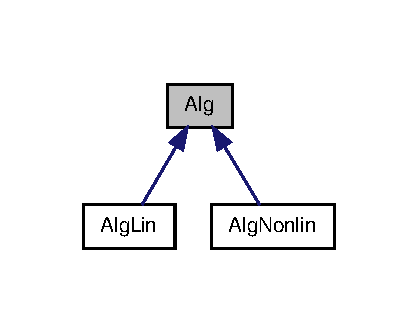
\includegraphics[width=200pt]{classAlg__inherit__graph}
\end{center}
\end{figure}
\subsection*{Public Member Functions}
\begin{DoxyCompactItemize}
\item 
\hyperlink{classAlg_a6c9a358be9a0b2cd2e35cf8a1ef6b60d}{Alg} (double in\_\-height, double in\_\-lenght, int in\_\-nx, int in\_\-ny, double in\_\-eps, char $\ast$in\_\-out\_\-name, int \hyperlink{classAlg_a919db7af2565185ba66adc8c0ae54686}{count}, double tau)
\begin{DoxyCompactList}\small\item\em Constructor. \end{DoxyCompactList}\item 
\hypertarget{classAlg_a21abd0bdf75af1e61e2c4dd00a5163f6}{
virtual void \hyperlink{classAlg_a21abd0bdf75af1e61e2c4dd00a5163f6}{resolve\_\-r} ()=0}
\label{classAlg_a21abd0bdf75af1e61e2c4dd00a5163f6}

\begin{DoxyCompactList}\small\item\em Recalculation of residuals for all equations. \end{DoxyCompactList}\item 
virtual void \hyperlink{classAlg_aa2436420b85976a48465408e9d86d425}{resolve\_\-r} (int mode)=0
\begin{DoxyCompactList}\small\item\em Recalculation of residuals for one equation. \end{DoxyCompactList}\item 
double \hyperlink{classAlg_abac775cccf3e4811358a05048a5300b2}{find\_\-coeff} (int name)
\begin{DoxyCompactList}\small\item\em Find iteration parameter. Is a wrapper for \char`\"{}find\char`\"{}. \end{DoxyCompactList}\item 
virtual double \hyperlink{classAlg_ada4ff3d2a0adb3b177d824e337158bfd}{find} (double $\ast$$\ast$a, double $\ast$$\ast$b, double $\ast$$\ast$c)=0
\begin{DoxyCompactList}\small\item\em Find iteration parameter.As changed algorythm of ALFA calculation, its implementation is moved to find with parameter \char`\"{}mode\char`\"{}. \end{DoxyCompactList}\item 
virtual double \hyperlink{classAlg_a979d6df06027c6353b682662d8c514fc}{find} (int mode, double $\ast$$\ast$a, double $\ast$$\ast$b, double $\ast$$\ast$c)=0
\begin{DoxyCompactList}\small\item\em Find iteration parameter for one equation. Used to find ALFA. \end{DoxyCompactList}\item 
virtual double $\ast$ \hyperlink{classAlg_aef9cdfe539aed53c23222715c551e11e}{find\_\-all} (double $\ast$$\ast$a, double $\ast$$\ast$b, double $\ast$$\ast$c)=0
\item 
\hypertarget{classAlg_a15c167548bbe12a4e021bfbb618faab0}{
virtual void \hyperlink{classAlg_a15c167548bbe12a4e021bfbb618faab0}{check\_\-result} ()=0}
\label{classAlg_a15c167548bbe12a4e021bfbb618faab0}

\begin{DoxyCompactList}\small\item\em Verify the calculation of residuals. \end{DoxyCompactList}\item 
void \hyperlink{classAlg_ad75df7e9510a1d765fdac3ab774144fb}{solve} (int out\_\-n)
\begin{DoxyCompactList}\small\item\em Main calculation loop by time. \end{DoxyCompactList}\item 
void \hyperlink{classAlg_a174f9ae3ac37adc830bf47b1829e2ddb}{resolve\_\-param} (double coeff, int name)
\begin{DoxyCompactList}\small\item\em Recalculation pov,u,v. Is a wrapper for resolve. \end{DoxyCompactList}\item 
void \hyperlink{classAlg_ad9daf68e4d275edab2d143b1fe9bf2e9}{resolve} (double coeff, double $\ast$$\ast$a, double $\ast$$\ast$b, double $\ast$$\ast$c)
\begin{DoxyCompactList}\small\item\em Recalculation pov,u,v with iteration parameter. After changing algorythm for ALFA, using for recaulculation with TAU. \end{DoxyCompactList}\item 
\hypertarget{classAlg_a693eaa5ee0a954e3907b0a3141b63925}{
void \hyperlink{classAlg_a693eaa5ee0a954e3907b0a3141b63925}{resolve\_\-for\_\-alfa} (double coeff, double $\ast$$\ast$a, double $\ast$$\ast$b, double $\ast$$\ast$c)}
\label{classAlg_a693eaa5ee0a954e3907b0a3141b63925}

\begin{DoxyCompactList}\small\item\em Deprecated for recalculation ALFA (now realized in resolve) \end{DoxyCompactList}\item 
double \hyperlink{classAlg_ab723793cded5d410eade7db32fe4a834}{diffX} (double $\ast$$\ast$a, int i, int j)
\begin{DoxyCompactList}\small\item\em differential analog of derivative by x \end{DoxyCompactList}\item 
double \hyperlink{classAlg_a986f8c7fc36030eda32e543d30d977ca}{diffY} (double $\ast$$\ast$a, int i, int j)
\begin{DoxyCompactList}\small\item\em differential analog of derivative by y \end{DoxyCompactList}\item 
double $\ast$$\ast$ \hyperlink{classAlg_a5763761a3053f1887e190633acccf0c2}{return\_\-pov} ()
\begin{DoxyCompactList}\small\item\em For access to pov from other threads. \end{DoxyCompactList}\item 
double $\ast$$\ast$ \hyperlink{classAlg_a94607ea61b791a6b6b468f15a1a090ab}{return\_\-u} ()
\begin{DoxyCompactList}\small\item\em For access to u from other threads. \end{DoxyCompactList}\item 
double $\ast$$\ast$ \hyperlink{classAlg_a181cf46ca43805230be57f7171ec9b55}{return\_\-v} ()
\begin{DoxyCompactList}\small\item\em For access to v from other threads. \end{DoxyCompactList}\item 
double \hyperlink{classAlg_a262fa430db2415621c8db3c5393e6258}{H} (int i, int j)
\begin{DoxyCompactList}\small\item\em Describe static function of bottom in point (i,j) \end{DoxyCompactList}\item 
double \hyperlink{classAlg_a3a4ae52d22f42babc6d6bf8759c27ec8}{B} (int i, int j, int \hyperlink{classAlg_a68d89159e07d755c5ec4235a10928674}{iter})
\begin{DoxyCompactList}\small\item\em Describe dynamic function of bottom in point (i,j) \end{DoxyCompactList}\item 
void \hyperlink{classAlg_a0fefea38317bcddeaa60b429eef2bdf3}{set\_\-temp} (int number)
\begin{DoxyCompactList}\small\item\em To set temporary (by time or method iterations) variables. \end{DoxyCompactList}\item 
double \hyperlink{classAlg_a3ccc4dd9b8720b025eaa4f10d139d2fb}{get\_\-norm\_\-r} ()
\begin{DoxyCompactList}\small\item\em Find residual norm. \end{DoxyCompactList}\item 
\hypertarget{classAlg_acfd3b6bba23d2fe8d0bb28ea7c7865a5}{
void \hyperlink{classAlg_acfd3b6bba23d2fe8d0bb28ea7c7865a5}{print} (double $\ast$$\ast$a, char $\ast$name)}
\label{classAlg_acfd3b6bba23d2fe8d0bb28ea7c7865a5}

\begin{DoxyCompactList}\small\item\em Deprecated function for printing (debug) \end{DoxyCompactList}\item 
\hypertarget{classAlg_a1cbe91213003b6fbc6930fdd474751c7}{
void \hyperlink{classAlg_a1cbe91213003b6fbc6930fdd474751c7}{print} (double $\ast$$\ast$a)}
\label{classAlg_a1cbe91213003b6fbc6930fdd474751c7}

\begin{DoxyCompactList}\small\item\em Deprecated function for printing (debug) \end{DoxyCompactList}\item 
\hypertarget{classAlg_a5b9211d86d4aa42b2d7eb3b259a82187}{
void \hyperlink{classAlg_a5b9211d86d4aa42b2d7eb3b259a82187}{print\_\-tec} (double $\ast$$\ast$a, char $\ast$out)}
\label{classAlg_a5b9211d86d4aa42b2d7eb3b259a82187}

\begin{DoxyCompactList}\small\item\em Deprecated function for printing (debug) \end{DoxyCompactList}\item 
void \hyperlink{classAlg_addc9b792b3fb548b12809952b46ad259}{set\_\-u\_\-v\_\-pov} (char $\ast$out\_\-u, char $\ast$out\_\-v, char $\ast$out\_\-pov)
\begin{DoxyCompactList}\small\item\em To set arbitrary initial data. \end{DoxyCompactList}\item 
void \hyperlink{classAlg_a28223f0814992218834e2d7a149b5b32}{set\_\-u\_\-v\_\-pov} (char $\ast$out\_\-u, char $\ast$out\_\-v)
\begin{DoxyCompactList}\small\item\em To set arbitrary initial data. \end{DoxyCompactList}\item 
\hypertarget{classAlg_a80fcd6f0678317828474af1282b51088}{
void \hyperlink{classAlg_a80fcd6f0678317828474af1282b51088}{set\_\-u\_\-v\_\-pov} ()}
\label{classAlg_a80fcd6f0678317828474af1282b51088}

\begin{DoxyCompactList}\small\item\em To set arbitrary initial data, which described by some function. \end{DoxyCompactList}\item 
\hypertarget{classAlg_a951b1131ee55c2ad043e438875f79c8b}{
void \hyperlink{classAlg_a951b1131ee55c2ad043e438875f79c8b}{get\_\-u\_\-v\_\-pov} (char $\ast$out\_\-u, char $\ast$out\_\-v, char $\ast$out\_\-pov)}
\label{classAlg_a951b1131ee55c2ad043e438875f79c8b}

\begin{DoxyCompactList}\small\item\em To output pov,u,v for future use in set\_\-u\_\-v\_\-pov. \end{DoxyCompactList}\item 
int \hyperlink{classAlg_ae2bdccac93c7a7e1b4ee22ee8b0634da}{getIter} ()
\begin{DoxyCompactList}\small\item\em For acces to iteration number from other threads. \end{DoxyCompactList}\item 
int \hyperlink{classAlg_aa377e54781d9fd7a3374dc64ede0d91d}{getCount} ()
\begin{DoxyCompactList}\small\item\em For acces to iteration count from other threads. \end{DoxyCompactList}\item 
double \hyperlink{classAlg_a5c2884279fc98cf7ea5f6e9893c86c61}{getMod} ()
\begin{DoxyCompactList}\small\item\em For acces to residual norm from other threads. \end{DoxyCompactList}\item 
void \hyperlink{classAlg_a48499068ba0c33ef77da2146f378cebf}{getH} (char $\ast$file\_\-name)
\begin{DoxyCompactList}\small\item\em Output bottom depth in file. \end{DoxyCompactList}\item 
\hypertarget{classAlg_ad1a45a2cb49f8d1a6d6cdaa37e8ce0ae}{
\hyperlink{classAlg_ad1a45a2cb49f8d1a6d6cdaa37e8ce0ae}{$\sim$Alg} ()}
\label{classAlg_ad1a45a2cb49f8d1a6d6cdaa37e8ce0ae}

\begin{DoxyCompactList}\small\item\em Dectructor. \end{DoxyCompactList}\end{DoxyCompactItemize}
\subsection*{Protected Attributes}
\begin{DoxyCompactItemize}
\item 
double $\ast$$\ast$ \hyperlink{classAlg_a91da00f3e2a7cef949da58b242d9305e}{pov}
\item 
double $\ast$$\ast$ \hyperlink{classAlg_a2f0a5afa848c3bfb1d8153e62aa434f6}{u}
\item 
double $\ast$$\ast$ \hyperlink{classAlg_a47f1cd35f394c7fafac69953e99274e0}{v}
\item 
double $\ast$$\ast$ \hyperlink{classAlg_ac6058a59828b5bb89532f37d84f4dfc2}{r1}
\item 
double $\ast$$\ast$ \hyperlink{classAlg_a5ca3705a31dd0a0f8e9e3b2455b63f3d}{r2}
\item 
double $\ast$$\ast$ \hyperlink{classAlg_af62c56e11f6523097ab3e1817da8453d}{r3}
\item 
double $\ast$$\ast$ \hyperlink{classAlg_adcdeccfa46eb9907962373371a2adb6b}{pov\_\-temp1}
\item 
double $\ast$$\ast$ \hyperlink{classAlg_ad60a4d85f33f58e39e026e608d8f3aa3}{u\_\-temp1}
\item 
double $\ast$$\ast$ \hyperlink{classAlg_a060c56407375b51f13bdfed2fe0b1e09}{v\_\-temp1}
\item 
double $\ast$$\ast$ \hyperlink{classAlg_aa6628cd62bd2c1e14311dada7d35ed6e}{pov\_\-temp2}
\item 
double $\ast$$\ast$ \hyperlink{classAlg_aa3a0ba123ec36f183c6f878cbc211c7f}{u\_\-temp2}
\item 
double $\ast$$\ast$ \hyperlink{classAlg_a1556924bbf451225dca91c36a7b65071}{v\_\-temp2}
\item 
\hypertarget{classAlg_a72316c58c79fa5494888fcfe4664e9d9}{
double $\ast$$\ast$ {\bfseries temp1}}
\label{classAlg_a72316c58c79fa5494888fcfe4664e9d9}

\item 
\hypertarget{classAlg_a1918cb7d719b4140d5ff445bfb1c97d8}{
double $\ast$$\ast$ {\bfseries temp2}}
\label{classAlg_a1918cb7d719b4140d5ff445bfb1c97d8}

\item 
\hypertarget{classAlg_ab97d547c5f23868d05e29db09e0a6db6}{
double $\ast$$\ast$ {\bfseries temp3}}
\label{classAlg_ab97d547c5f23868d05e29db09e0a6db6}

\item 
double $\ast$$\ast$ \hyperlink{classAlg_ad2f2df479bdee0b098e959eb6750ad24}{HBu}
\item 
double $\ast$$\ast$ \hyperlink{classAlg_abf4332341084e55c633251179030c52f}{HBv}
\item 
double $\ast$$\ast$ \hyperlink{classAlg_a1ab7953aa405a7f650e000fffa446ca1}{uu}
\item 
double $\ast$$\ast$ \hyperlink{classAlg_a39918c7b3ec73091844aaa16482b60bc}{vv}
\item 
double $\ast$$\ast$ \hyperlink{classAlg_a151c5a0de6551e528f886addad8cf9f3}{HBb}
\item 
double $\ast$$\ast$ \hyperlink{classAlg_a68d9a231e894287711a457005962e835}{HBc}
\item 
double $\ast$$\ast$ \hyperlink{classAlg_a325514811e51f84c9f45d910f61cd57b}{bb}
\item 
double $\ast$$\ast$ \hyperlink{classAlg_a80d1cd9b48cd0e83fadbb02058e889c2}{cc}
\item 
double $\ast$$\ast$ \hyperlink{classAlg_abe075d41b8b6c5d13788d18cbc0abb13}{z}
\item 
double $\ast$$\ast$ \hyperlink{classAlg_a243ec21fdadb52db5eb1908f6ac2b493}{check1}
\item 
double $\ast$$\ast$ \hyperlink{classAlg_a133497b0dd41c024c1cb3278903c69ff}{check2}
\item 
double $\ast$$\ast$ \hyperlink{classAlg_a595d62a49951a021c9cc071f0079a21a}{check3}
\item 
double \hyperlink{classAlg_a60c5daa9c7917681e7ef07f912dabbb5}{height}
\item 
\hypertarget{classAlg_a9c630456c790085e0daac3313e2525b6}{
double {\bfseries lenght}}
\label{classAlg_a9c630456c790085e0daac3313e2525b6}

\item 
int \hyperlink{classAlg_a3d223cee974b6928608b0975e406bc5c}{nx}
\item 
\hypertarget{classAlg_a43ae4b87276544104c1211817a8783f8}{
int {\bfseries ny}}
\label{classAlg_a43ae4b87276544104c1211817a8783f8}

\item 
double \hyperlink{classAlg_a7baeb3f5e56097c1bcd1bdd7c248748a}{hx}
\item 
\hypertarget{classAlg_abd9ad8f0ad3f50a5da3cf6e75fbb940e}{
double {\bfseries hy}}
\label{classAlg_abd9ad8f0ad3f50a5da3cf6e75fbb940e}

\item 
\hypertarget{classAlg_aadc1b035b9e8dfa7d3a9670b77bc8280}{
double {\bfseries t}}
\label{classAlg_aadc1b035b9e8dfa7d3a9670b77bc8280}

\item 
int \hyperlink{classAlg_a68d89159e07d755c5ec4235a10928674}{iter}
\item 
double \hyperlink{classAlg_aacfa2077c54f2971b335927ef4e952c8}{eps}
\item 
char \hyperlink{classAlg_a57e8fa04c6ffb36bb472077251682493}{out\_\-name} \mbox{[}256\mbox{]}
\item 
int \hyperlink{classAlg_a919db7af2565185ba66adc8c0ae54686}{count}
\item 
double \hyperlink{classAlg_a48f35bad3ab97c5bbabb1ecf572980e1}{mod}
\item 
\hypertarget{classAlg_a5456c37cc79b3b4599421034770bfe47}{
double {\bfseries a1}}
\label{classAlg_a5456c37cc79b3b4599421034770bfe47}

\item 
\hypertarget{classAlg_a4e01d2438ed834ec2e907a76225ef6c9}{
double {\bfseries a2}}
\label{classAlg_a4e01d2438ed834ec2e907a76225ef6c9}

\item 
\hypertarget{classAlg_aa7c6cd580b013334b155470c16487b85}{
double {\bfseries a3}}
\label{classAlg_aa7c6cd580b013334b155470c16487b85}

\item 
\hypertarget{classAlg_a18ce9365df4d088e54a47175f8abc298}{
int {\bfseries count\_\-a1}}
\label{classAlg_a18ce9365df4d088e54a47175f8abc298}

\item 
\hypertarget{classAlg_ac53103a2592938146864e8d0417ca334}{
int {\bfseries count\_\-a2}}
\label{classAlg_ac53103a2592938146864e8d0417ca334}

\item 
\hypertarget{classAlg_a382a13f475dc2ef8b44637d26cf5af2a}{
int {\bfseries count\_\-a3}}
\label{classAlg_a382a13f475dc2ef8b44637d26cf5af2a}

\item 
\hypertarget{classAlg_adc69cc8818bcc5c1edca9c2d987385d4}{
FILE $\ast$ {\bfseries log}}
\label{classAlg_adc69cc8818bcc5c1edca9c2d987385d4}

\end{DoxyCompactItemize}


\subsection{Detailed Description}
Base class for calculation  This class contains general functional and abstract realization algorythm. 

\subsection{Constructor \& Destructor Documentation}
\hypertarget{classAlg_a6c9a358be9a0b2cd2e35cf8a1ef6b60d}{
\index{Alg@{Alg}!Alg@{Alg}}
\index{Alg@{Alg}!Alg@{Alg}}
\subsubsection[{Alg}]{\setlength{\rightskip}{0pt plus 5cm}Alg::Alg (
\begin{DoxyParamCaption}
\item[{double}]{in\_\-height, }
\item[{double}]{in\_\-lenght, }
\item[{int}]{in\_\-nx, }
\item[{int}]{in\_\-ny, }
\item[{double}]{in\_\-eps, }
\item[{char $\ast$}]{in\_\-out\_\-name, }
\item[{int}]{count, }
\item[{double}]{tau}
\end{DoxyParamCaption}
)}}
\label{classAlg_a6c9a358be9a0b2cd2e35cf8a1ef6b60d}


Constructor. 


\begin{DoxyParams}{Parameters}
{\em in\_\-height} & Height calculation area \\
\hline
{\em in\_\-lenght} & Lenght calculation area \\
\hline
{\em in\_\-nx} & Count of Ox node \\
\hline
{\em in\_\-ny} & Count of Oy node \\
\hline
{\em in\_\-eps} & The accuracy of calculations \\
\hline
{\em in\_\-out\_\-name} & Output filename for save result \\
\hline
{\em count} & Count iteration by time \\
\hline
{\em tau} & Strp by time \\
\hline
\end{DoxyParams}


set initial state



\subsection{Member Function Documentation}
\hypertarget{classAlg_a3a4ae52d22f42babc6d6bf8759c27ec8}{
\index{Alg@{Alg}!B@{B}}
\index{B@{B}!Alg@{Alg}}
\subsubsection[{B}]{\setlength{\rightskip}{0pt plus 5cm}double Alg::B (
\begin{DoxyParamCaption}
\item[{int}]{i, }
\item[{int}]{j, }
\item[{int}]{iter}
\end{DoxyParamCaption}
)\hspace{0.3cm}{\ttfamily  \mbox{[}inline\mbox{]}}}}
\label{classAlg_a3a4ae52d22f42babc6d6bf8759c27ec8}


Describe dynamic function of bottom in point (i,j) 


\begin{DoxyParams}{Parameters}
{\em i} & Node number \\
\hline
{\em j} & Node number \\
\hline
\end{DoxyParams}
\begin{DoxyReturn}{Returns}
Bottom depth 
\end{DoxyReturn}
\hypertarget{classAlg_ab723793cded5d410eade7db32fe4a834}{
\index{Alg@{Alg}!diffX@{diffX}}
\index{diffX@{diffX}!Alg@{Alg}}
\subsubsection[{diffX}]{\setlength{\rightskip}{0pt plus 5cm}double Alg::diffX (
\begin{DoxyParamCaption}
\item[{double $\ast$$\ast$}]{a, }
\item[{int}]{i, }
\item[{int}]{j}
\end{DoxyParamCaption}
)\hspace{0.3cm}{\ttfamily  \mbox{[}inline\mbox{]}}}}
\label{classAlg_ab723793cded5d410eade7db32fe4a834}


differential analog of derivative by x 


\begin{DoxyParams}{Parameters}
{\em a} & variable which used for derivation \\
\hline
{\em i} & node number (for check boundaries) \\
\hline
{\em j} & node number (for check boundaries) \\
\hline
\end{DoxyParams}
\hypertarget{classAlg_a986f8c7fc36030eda32e543d30d977ca}{
\index{Alg@{Alg}!diffY@{diffY}}
\index{diffY@{diffY}!Alg@{Alg}}
\subsubsection[{diffY}]{\setlength{\rightskip}{0pt plus 5cm}double Alg::diffY (
\begin{DoxyParamCaption}
\item[{double $\ast$$\ast$}]{a, }
\item[{int}]{i, }
\item[{int}]{j}
\end{DoxyParamCaption}
)\hspace{0.3cm}{\ttfamily  \mbox{[}inline\mbox{]}}}}
\label{classAlg_a986f8c7fc36030eda32e543d30d977ca}


differential analog of derivative by y 


\begin{DoxyParams}{Parameters}
{\em a} & variable which used for derivation \\
\hline
{\em i} & node number (for check boundaries) \\
\hline
{\em j} & node number (for check boundaries) \\
\hline
\end{DoxyParams}
\hypertarget{classAlg_a979d6df06027c6353b682662d8c514fc}{
\index{Alg@{Alg}!find@{find}}
\index{find@{find}!Alg@{Alg}}
\subsubsection[{find}]{\setlength{\rightskip}{0pt plus 5cm}virtual double Alg::find (
\begin{DoxyParamCaption}
\item[{int}]{mode, }
\item[{double $\ast$$\ast$}]{a, }
\item[{double $\ast$$\ast$}]{b, }
\item[{double $\ast$$\ast$}]{c}
\end{DoxyParamCaption}
)\hspace{0.3cm}{\ttfamily  \mbox{[}pure virtual\mbox{]}}}}
\label{classAlg_a979d6df06027c6353b682662d8c514fc}


Find iteration parameter for one equation. Used to find ALFA. 


\begin{DoxyParams}{Parameters}
{\em mode} & Number of equations, for which coefficient searched \\
\hline
{\em a} & First data array for operator (to find ALFA -\/-\/ z) \\
\hline
{\em b} & Second data array for operator (to find ALFA -\/-\/ z) \\
\hline
{\em c} & Third data array for operator (to find ALFA -\/-\/ z) \\
\hline
\end{DoxyParams}
\begin{DoxyReturn}{Returns}
Iteration parameter (ALFA) 
\end{DoxyReturn}


Implemented in \hyperlink{classAlgLin_a0e6a96c3b072cb277bd7b1d4dd945472}{AlgLin}, and \hyperlink{classAlgNonlin_a164094279ad86962c650221b112c9223}{AlgNonlin}.

\hypertarget{classAlg_ada4ff3d2a0adb3b177d824e337158bfd}{
\index{Alg@{Alg}!find@{find}}
\index{find@{find}!Alg@{Alg}}
\subsubsection[{find}]{\setlength{\rightskip}{0pt plus 5cm}virtual double Alg::find (
\begin{DoxyParamCaption}
\item[{double $\ast$$\ast$}]{a, }
\item[{double $\ast$$\ast$}]{b, }
\item[{double $\ast$$\ast$}]{c}
\end{DoxyParamCaption}
)\hspace{0.3cm}{\ttfamily  \mbox{[}pure virtual\mbox{]}}}}
\label{classAlg_ada4ff3d2a0adb3b177d824e337158bfd}


Find iteration parameter.As changed algorythm of ALFA calculation, its implementation is moved to find with parameter \char`\"{}mode\char`\"{}. 


\begin{DoxyParams}{Parameters}
{\em a} & First data array for operator (to find TAU -\/-\/ pov) \\
\hline
{\em b} & Second data array for operator (to find TAU -\/-\/ u) \\
\hline
{\em c} & Third data array for operator (to find TAU -\/-\/ v) \\
\hline
\end{DoxyParams}
\begin{DoxyReturn}{Returns}
Iteration parameter (TAU) 
\end{DoxyReturn}


Implemented in \hyperlink{classAlgLin_a8323f1f45960e8d39184a61730fffffb}{AlgLin}, and \hyperlink{classAlgNonlin_ae7c521438daed488cd69b131292f2a8a}{AlgNonlin}.

\hypertarget{classAlg_aef9cdfe539aed53c23222715c551e11e}{
\index{Alg@{Alg}!find\_\-all@{find\_\-all}}
\index{find\_\-all@{find\_\-all}!Alg@{Alg}}
\subsubsection[{find\_\-all}]{\setlength{\rightskip}{0pt plus 5cm}virtual double$\ast$ Alg::find\_\-all (
\begin{DoxyParamCaption}
\item[{double $\ast$$\ast$}]{a, }
\item[{double $\ast$$\ast$}]{b, }
\item[{double $\ast$$\ast$}]{c}
\end{DoxyParamCaption}
)\hspace{0.3cm}{\ttfamily  \mbox{[}pure virtual\mbox{]}}}}
\label{classAlg_aef9cdfe539aed53c23222715c551e11e}
Deprecated method for calculation ALFA 

Implemented in \hyperlink{classAlgLin_ac5e5cd276c5be663d2d36ab92bf6ad83}{AlgLin}, and \hyperlink{classAlgNonlin_a3f3bdece3eb2ccaffeb7c19bd318121e}{AlgNonlin}.

\hypertarget{classAlg_abac775cccf3e4811358a05048a5300b2}{
\index{Alg@{Alg}!find\_\-coeff@{find\_\-coeff}}
\index{find\_\-coeff@{find\_\-coeff}!Alg@{Alg}}
\subsubsection[{find\_\-coeff}]{\setlength{\rightskip}{0pt plus 5cm}double Alg::find\_\-coeff (
\begin{DoxyParamCaption}
\item[{int}]{name}
\end{DoxyParamCaption}
)}}
\label{classAlg_abac775cccf3e4811358a05048a5300b2}


Find iteration parameter. Is a wrapper for \char`\"{}find\char`\"{}. 


\begin{DoxyParams}{Parameters}
{\em name} & Name of iteration parameter (now used to find only TAU) \\
\hline
\end{DoxyParams}
\begin{DoxyReturn}{Returns}
Iteration parameter (TAU) 
\end{DoxyReturn}
\hypertarget{classAlg_a3ccc4dd9b8720b025eaa4f10d139d2fb}{
\index{Alg@{Alg}!get\_\-norm\_\-r@{get\_\-norm\_\-r}}
\index{get\_\-norm\_\-r@{get\_\-norm\_\-r}!Alg@{Alg}}
\subsubsection[{get\_\-norm\_\-r}]{\setlength{\rightskip}{0pt plus 5cm}double Alg::get\_\-norm\_\-r (
\begin{DoxyParamCaption}
{}
\end{DoxyParamCaption}
)}}
\label{classAlg_a3ccc4dd9b8720b025eaa4f10d139d2fb}


Find residual norm. 

\begin{DoxyReturn}{Returns}
Residual norm 
\end{DoxyReturn}
\hypertarget{classAlg_aa377e54781d9fd7a3374dc64ede0d91d}{
\index{Alg@{Alg}!getCount@{getCount}}
\index{getCount@{getCount}!Alg@{Alg}}
\subsubsection[{getCount}]{\setlength{\rightskip}{0pt plus 5cm}int Alg::getCount (
\begin{DoxyParamCaption}
{}
\end{DoxyParamCaption}
)}}
\label{classAlg_aa377e54781d9fd7a3374dc64ede0d91d}


For acces to iteration count from other threads. 

\begin{DoxyReturn}{Returns}
iteration count 
\end{DoxyReturn}
\hypertarget{classAlg_a48499068ba0c33ef77da2146f378cebf}{
\index{Alg@{Alg}!getH@{getH}}
\index{getH@{getH}!Alg@{Alg}}
\subsubsection[{getH}]{\setlength{\rightskip}{0pt plus 5cm}void Alg::getH (
\begin{DoxyParamCaption}
\item[{char $\ast$}]{file\_\-name}
\end{DoxyParamCaption}
)}}
\label{classAlg_a48499068ba0c33ef77da2146f378cebf}


Output bottom depth in file. 


\begin{DoxyParams}{Parameters}
{\em file\_\-name} & Output file name \\
\hline
\end{DoxyParams}


output in file -\/H!

\hypertarget{classAlg_ae2bdccac93c7a7e1b4ee22ee8b0634da}{
\index{Alg@{Alg}!getIter@{getIter}}
\index{getIter@{getIter}!Alg@{Alg}}
\subsubsection[{getIter}]{\setlength{\rightskip}{0pt plus 5cm}int Alg::getIter (
\begin{DoxyParamCaption}
{}
\end{DoxyParamCaption}
)}}
\label{classAlg_ae2bdccac93c7a7e1b4ee22ee8b0634da}


For acces to iteration number from other threads. 

\begin{DoxyReturn}{Returns}
iteration number 
\end{DoxyReturn}
\hypertarget{classAlg_a5c2884279fc98cf7ea5f6e9893c86c61}{
\index{Alg@{Alg}!getMod@{getMod}}
\index{getMod@{getMod}!Alg@{Alg}}
\subsubsection[{getMod}]{\setlength{\rightskip}{0pt plus 5cm}double Alg::getMod (
\begin{DoxyParamCaption}
{}
\end{DoxyParamCaption}
)}}
\label{classAlg_a5c2884279fc98cf7ea5f6e9893c86c61}


For acces to residual norm from other threads. 

\begin{DoxyReturn}{Returns}
residual norm 
\end{DoxyReturn}
\hypertarget{classAlg_a262fa430db2415621c8db3c5393e6258}{
\index{Alg@{Alg}!H@{H}}
\index{H@{H}!Alg@{Alg}}
\subsubsection[{H}]{\setlength{\rightskip}{0pt plus 5cm}double Alg::H (
\begin{DoxyParamCaption}
\item[{int}]{i, }
\item[{int}]{j}
\end{DoxyParamCaption}
)\hspace{0.3cm}{\ttfamily  \mbox{[}inline\mbox{]}}}}
\label{classAlg_a262fa430db2415621c8db3c5393e6258}


Describe static function of bottom in point (i,j) 


\begin{DoxyParams}{Parameters}
{\em i} & Node number \\
\hline
{\em j} & Node number \\
\hline
\end{DoxyParams}
\begin{DoxyReturn}{Returns}
Bottom depth 
\end{DoxyReturn}
\hypertarget{classAlg_ad9daf68e4d275edab2d143b1fe9bf2e9}{
\index{Alg@{Alg}!resolve@{resolve}}
\index{resolve@{resolve}!Alg@{Alg}}
\subsubsection[{resolve}]{\setlength{\rightskip}{0pt plus 5cm}void Alg::resolve (
\begin{DoxyParamCaption}
\item[{double}]{coeff, }
\item[{double $\ast$$\ast$}]{a, }
\item[{double $\ast$$\ast$}]{b, }
\item[{double $\ast$$\ast$}]{c}
\end{DoxyParamCaption}
)}}
\label{classAlg_ad9daf68e4d275edab2d143b1fe9bf2e9}


Recalculation pov,u,v with iteration parameter. After changing algorythm for ALFA, using for recaulculation with TAU. 


\begin{DoxyParams}{Parameters}
{\em coeff} & Value of iteration parameter \\
\hline
{\em a} & First data array (for TAU -\/ pov) \\
\hline
{\em b} & Second data array (for TAU -\/ u) \\
\hline
{\em c} & Third data array (for TAU -\/ v) \\
\hline
\end{DoxyParams}
\hypertarget{classAlg_a174f9ae3ac37adc830bf47b1829e2ddb}{
\index{Alg@{Alg}!resolve\_\-param@{resolve\_\-param}}
\index{resolve\_\-param@{resolve\_\-param}!Alg@{Alg}}
\subsubsection[{resolve\_\-param}]{\setlength{\rightskip}{0pt plus 5cm}void Alg::resolve\_\-param (
\begin{DoxyParamCaption}
\item[{double}]{coeff, }
\item[{int}]{name}
\end{DoxyParamCaption}
)}}
\label{classAlg_a174f9ae3ac37adc830bf47b1829e2ddb}


Recalculation pov,u,v. Is a wrapper for resolve. 


\begin{DoxyParams}{Parameters}
{\em coeff} & Iteration coefficient (now using only for TAU) \\
\hline
{\em name} & Name of iteration coefficient (TAU or ALFA) \\
\hline
\end{DoxyParams}
\hypertarget{classAlg_aa2436420b85976a48465408e9d86d425}{
\index{Alg@{Alg}!resolve\_\-r@{resolve\_\-r}}
\index{resolve\_\-r@{resolve\_\-r}!Alg@{Alg}}
\subsubsection[{resolve\_\-r}]{\setlength{\rightskip}{0pt plus 5cm}virtual void Alg::resolve\_\-r (
\begin{DoxyParamCaption}
\item[{int}]{mode}
\end{DoxyParamCaption}
)\hspace{0.3cm}{\ttfamily  \mbox{[}pure virtual\mbox{]}}}}
\label{classAlg_aa2436420b85976a48465408e9d86d425}


Recalculation of residuals for one equation. 


\begin{DoxyParams}{Parameters}
{\em mode} & Number of equation for recalculation \\
\hline
\end{DoxyParams}


Implemented in \hyperlink{classAlgLin_a7784f0707d7a081da5f85615f374df32}{AlgLin}, and \hyperlink{classAlgNonlin_a28bbb13e708a32cf4f191db56325e52c}{AlgNonlin}.

\hypertarget{classAlg_a5763761a3053f1887e190633acccf0c2}{
\index{Alg@{Alg}!return\_\-pov@{return\_\-pov}}
\index{return\_\-pov@{return\_\-pov}!Alg@{Alg}}
\subsubsection[{return\_\-pov}]{\setlength{\rightskip}{0pt plus 5cm}double$\ast$$\ast$ Alg::return\_\-pov (
\begin{DoxyParamCaption}
{}
\end{DoxyParamCaption}
)\hspace{0.3cm}{\ttfamily  \mbox{[}inline\mbox{]}}}}
\label{classAlg_a5763761a3053f1887e190633acccf0c2}


For access to pov from other threads. 

\begin{DoxyReturn}{Returns}
pov 
\end{DoxyReturn}
\hypertarget{classAlg_a94607ea61b791a6b6b468f15a1a090ab}{
\index{Alg@{Alg}!return\_\-u@{return\_\-u}}
\index{return\_\-u@{return\_\-u}!Alg@{Alg}}
\subsubsection[{return\_\-u}]{\setlength{\rightskip}{0pt plus 5cm}double$\ast$$\ast$ Alg::return\_\-u (
\begin{DoxyParamCaption}
{}
\end{DoxyParamCaption}
)\hspace{0.3cm}{\ttfamily  \mbox{[}inline\mbox{]}}}}
\label{classAlg_a94607ea61b791a6b6b468f15a1a090ab}


For access to u from other threads. 

\begin{DoxyReturn}{Returns}
u 
\end{DoxyReturn}
\hypertarget{classAlg_a181cf46ca43805230be57f7171ec9b55}{
\index{Alg@{Alg}!return\_\-v@{return\_\-v}}
\index{return\_\-v@{return\_\-v}!Alg@{Alg}}
\subsubsection[{return\_\-v}]{\setlength{\rightskip}{0pt plus 5cm}double$\ast$$\ast$ Alg::return\_\-v (
\begin{DoxyParamCaption}
{}
\end{DoxyParamCaption}
)\hspace{0.3cm}{\ttfamily  \mbox{[}inline\mbox{]}}}}
\label{classAlg_a181cf46ca43805230be57f7171ec9b55}


For access to v from other threads. 

\begin{DoxyReturn}{Returns}
v 
\end{DoxyReturn}
\hypertarget{classAlg_a0fefea38317bcddeaa60b429eef2bdf3}{
\index{Alg@{Alg}!set\_\-temp@{set\_\-temp}}
\index{set\_\-temp@{set\_\-temp}!Alg@{Alg}}
\subsubsection[{set\_\-temp}]{\setlength{\rightskip}{0pt plus 5cm}void Alg::set\_\-temp (
\begin{DoxyParamCaption}
\item[{int}]{number}
\end{DoxyParamCaption}
)}}
\label{classAlg_a0fefea38317bcddeaa60b429eef2bdf3}


To set temporary (by time or method iterations) variables. 


\begin{DoxyParams}{Parameters}
{\em number} & If set pov\_\-temp1,u\_\-temp1,v\_\-temp1 -\/ 0. If set pov\_\-temp2,u\_\-temp2\_\-v\_\-temp2 -\/ 1. \\
\hline
\end{DoxyParams}
\hypertarget{classAlg_a28223f0814992218834e2d7a149b5b32}{
\index{Alg@{Alg}!set\_\-u\_\-v\_\-pov@{set\_\-u\_\-v\_\-pov}}
\index{set\_\-u\_\-v\_\-pov@{set\_\-u\_\-v\_\-pov}!Alg@{Alg}}
\subsubsection[{set\_\-u\_\-v\_\-pov}]{\setlength{\rightskip}{0pt plus 5cm}void Alg::set\_\-u\_\-v\_\-pov (
\begin{DoxyParamCaption}
\item[{char $\ast$}]{out\_\-u, }
\item[{char $\ast$}]{out\_\-v}
\end{DoxyParamCaption}
)}}
\label{classAlg_a28223f0814992218834e2d7a149b5b32}


To set arbitrary initial data. 


\begin{DoxyParams}{Parameters}
{\em out\_\-u} & Path to file with u data \\
\hline
{\em out\_\-v} & Path to file with v data \\
\hline
\end{DoxyParams}
\hypertarget{classAlg_addc9b792b3fb548b12809952b46ad259}{
\index{Alg@{Alg}!set\_\-u\_\-v\_\-pov@{set\_\-u\_\-v\_\-pov}}
\index{set\_\-u\_\-v\_\-pov@{set\_\-u\_\-v\_\-pov}!Alg@{Alg}}
\subsubsection[{set\_\-u\_\-v\_\-pov}]{\setlength{\rightskip}{0pt plus 5cm}void Alg::set\_\-u\_\-v\_\-pov (
\begin{DoxyParamCaption}
\item[{char $\ast$}]{out\_\-u, }
\item[{char $\ast$}]{out\_\-v, }
\item[{char $\ast$}]{out\_\-pov}
\end{DoxyParamCaption}
)}}
\label{classAlg_addc9b792b3fb548b12809952b46ad259}


To set arbitrary initial data. 


\begin{DoxyParams}{Parameters}
{\em out\_\-u} & Path to file with u data \\
\hline
{\em out\_\-v} & Path to file with v data \\
\hline
{\em out\_\-pov} & Path to file with pov data \\
\hline
\end{DoxyParams}
\hypertarget{classAlg_ad75df7e9510a1d765fdac3ab774144fb}{
\index{Alg@{Alg}!solve@{solve}}
\index{solve@{solve}!Alg@{Alg}}
\subsubsection[{solve}]{\setlength{\rightskip}{0pt plus 5cm}void Alg::solve (
\begin{DoxyParamCaption}
\item[{int}]{out\_\-n}
\end{DoxyParamCaption}
)}}
\label{classAlg_ad75df7e9510a1d765fdac3ab774144fb}


Main calculation loop by time. 


\begin{DoxyParams}{Parameters}
{\em out\_\-n} & Frequency of write result on disk (for large calculations) \\
\hline
\end{DoxyParams}


create printing thread



\subsection{Member Data Documentation}
\hypertarget{classAlg_a325514811e51f84c9f45d910f61cd57b}{
\index{Alg@{Alg}!bb@{bb}}
\index{bb@{bb}!Alg@{Alg}}
\subsubsection[{bb}]{\setlength{\rightskip}{0pt plus 5cm}double$\ast$$\ast$ {\bf Alg::bb}\hspace{0.3cm}{\ttfamily  \mbox{[}protected\mbox{]}}}}
\label{classAlg_a325514811e51f84c9f45d910f61cd57b}
temporary for solving (placed here only for optimize memory allocation) \hypertarget{classAlg_a80d1cd9b48cd0e83fadbb02058e889c2}{
\index{Alg@{Alg}!cc@{cc}}
\index{cc@{cc}!Alg@{Alg}}
\subsubsection[{cc}]{\setlength{\rightskip}{0pt plus 5cm}double$\ast$$\ast$ {\bf Alg::cc}\hspace{0.3cm}{\ttfamily  \mbox{[}protected\mbox{]}}}}
\label{classAlg_a80d1cd9b48cd0e83fadbb02058e889c2}
temporary for solving (placed here only for optimize memory allocation) \hypertarget{classAlg_a243ec21fdadb52db5eb1908f6ac2b493}{
\index{Alg@{Alg}!check1@{check1}}
\index{check1@{check1}!Alg@{Alg}}
\subsubsection[{check1}]{\setlength{\rightskip}{0pt plus 5cm}double$\ast$$\ast$ {\bf Alg::check1}\hspace{0.3cm}{\ttfamily  \mbox{[}protected\mbox{]}}}}
\label{classAlg_a243ec21fdadb52db5eb1908f6ac2b493}
for checking(debug) \hypertarget{classAlg_a133497b0dd41c024c1cb3278903c69ff}{
\index{Alg@{Alg}!check2@{check2}}
\index{check2@{check2}!Alg@{Alg}}
\subsubsection[{check2}]{\setlength{\rightskip}{0pt plus 5cm}double$\ast$$\ast$ {\bf Alg::check2}\hspace{0.3cm}{\ttfamily  \mbox{[}protected\mbox{]}}}}
\label{classAlg_a133497b0dd41c024c1cb3278903c69ff}
for checking(debug) \hypertarget{classAlg_a595d62a49951a021c9cc071f0079a21a}{
\index{Alg@{Alg}!check3@{check3}}
\index{check3@{check3}!Alg@{Alg}}
\subsubsection[{check3}]{\setlength{\rightskip}{0pt plus 5cm}double$\ast$$\ast$ {\bf Alg::check3}\hspace{0.3cm}{\ttfamily  \mbox{[}protected\mbox{]}}}}
\label{classAlg_a595d62a49951a021c9cc071f0079a21a}
for checking(debug) \hypertarget{classAlg_a919db7af2565185ba66adc8c0ae54686}{
\index{Alg@{Alg}!count@{count}}
\index{count@{count}!Alg@{Alg}}
\subsubsection[{count}]{\setlength{\rightskip}{0pt plus 5cm}int {\bf Alg::count}\hspace{0.3cm}{\ttfamily  \mbox{[}protected\mbox{]}}}}
\label{classAlg_a919db7af2565185ba66adc8c0ae54686}
Count steps by time \hypertarget{classAlg_aacfa2077c54f2971b335927ef4e952c8}{
\index{Alg@{Alg}!eps@{eps}}
\index{eps@{eps}!Alg@{Alg}}
\subsubsection[{eps}]{\setlength{\rightskip}{0pt plus 5cm}double {\bf Alg::eps}\hspace{0.3cm}{\ttfamily  \mbox{[}protected\mbox{]}}}}
\label{classAlg_aacfa2077c54f2971b335927ef4e952c8}
Presice of method of incomplete approximation of minimal reciduals \hypertarget{classAlg_a151c5a0de6551e528f886addad8cf9f3}{
\index{Alg@{Alg}!HBb@{HBb}}
\index{HBb@{HBb}!Alg@{Alg}}
\subsubsection[{HBb}]{\setlength{\rightskip}{0pt plus 5cm}double$\ast$$\ast$ {\bf Alg::HBb}\hspace{0.3cm}{\ttfamily  \mbox{[}protected\mbox{]}}}}
\label{classAlg_a151c5a0de6551e528f886addad8cf9f3}
temporary for solving (placed here only for optimize memory allocation) \hypertarget{classAlg_a68d9a231e894287711a457005962e835}{
\index{Alg@{Alg}!HBc@{HBc}}
\index{HBc@{HBc}!Alg@{Alg}}
\subsubsection[{HBc}]{\setlength{\rightskip}{0pt plus 5cm}double$\ast$$\ast$ {\bf Alg::HBc}\hspace{0.3cm}{\ttfamily  \mbox{[}protected\mbox{]}}}}
\label{classAlg_a68d9a231e894287711a457005962e835}
temporary for solving (placed here only for optimize memory allocation) \hypertarget{classAlg_ad2f2df479bdee0b098e959eb6750ad24}{
\index{Alg@{Alg}!HBu@{HBu}}
\index{HBu@{HBu}!Alg@{Alg}}
\subsubsection[{HBu}]{\setlength{\rightskip}{0pt plus 5cm}double$\ast$$\ast$ {\bf Alg::HBu}\hspace{0.3cm}{\ttfamily  \mbox{[}protected\mbox{]}}}}
\label{classAlg_ad2f2df479bdee0b098e959eb6750ad24}
temporary for solving (placed here only for optimize memory allocation) \hypertarget{classAlg_abf4332341084e55c633251179030c52f}{
\index{Alg@{Alg}!HBv@{HBv}}
\index{HBv@{HBv}!Alg@{Alg}}
\subsubsection[{HBv}]{\setlength{\rightskip}{0pt plus 5cm}double$\ast$$\ast$ {\bf Alg::HBv}\hspace{0.3cm}{\ttfamily  \mbox{[}protected\mbox{]}}}}
\label{classAlg_abf4332341084e55c633251179030c52f}
temporary for solving (placed here only for optimize memory allocation) \hypertarget{classAlg_a60c5daa9c7917681e7ef07f912dabbb5}{
\index{Alg@{Alg}!height@{height}}
\index{height@{height}!Alg@{Alg}}
\subsubsection[{height}]{\setlength{\rightskip}{0pt plus 5cm}double {\bf Alg::height}\hspace{0.3cm}{\ttfamily  \mbox{[}protected\mbox{]}}}}
\label{classAlg_a60c5daa9c7917681e7ef07f912dabbb5}
Area parameters \hypertarget{classAlg_a7baeb3f5e56097c1bcd1bdd7c248748a}{
\index{Alg@{Alg}!hx@{hx}}
\index{hx@{hx}!Alg@{Alg}}
\subsubsection[{hx}]{\setlength{\rightskip}{0pt plus 5cm}double {\bf Alg::hx}\hspace{0.3cm}{\ttfamily  \mbox{[}protected\mbox{]}}}}
\label{classAlg_a7baeb3f5e56097c1bcd1bdd7c248748a}
Steps by space/time \hypertarget{classAlg_a68d89159e07d755c5ec4235a10928674}{
\index{Alg@{Alg}!iter@{iter}}
\index{iter@{iter}!Alg@{Alg}}
\subsubsection[{iter}]{\setlength{\rightskip}{0pt plus 5cm}int {\bf Alg::iter}\hspace{0.3cm}{\ttfamily  \mbox{[}protected\mbox{]}}}}
\label{classAlg_a68d89159e07d755c5ec4235a10928674}
Current iteration \hypertarget{classAlg_a48f35bad3ab97c5bbabb1ecf572980e1}{
\index{Alg@{Alg}!mod@{mod}}
\index{mod@{mod}!Alg@{Alg}}
\subsubsection[{mod}]{\setlength{\rightskip}{0pt plus 5cm}double {\bf Alg::mod}\hspace{0.3cm}{\ttfamily  \mbox{[}protected\mbox{]}}}}
\label{classAlg_a48f35bad3ab97c5bbabb1ecf572980e1}
Norm of reciduals \hypertarget{classAlg_a3d223cee974b6928608b0975e406bc5c}{
\index{Alg@{Alg}!nx@{nx}}
\index{nx@{nx}!Alg@{Alg}}
\subsubsection[{nx}]{\setlength{\rightskip}{0pt plus 5cm}int {\bf Alg::nx}\hspace{0.3cm}{\ttfamily  \mbox{[}protected\mbox{]}}}}
\label{classAlg_a3d223cee974b6928608b0975e406bc5c}
Num of nodes \hypertarget{classAlg_a57e8fa04c6ffb36bb472077251682493}{
\index{Alg@{Alg}!out\_\-name@{out\_\-name}}
\index{out\_\-name@{out\_\-name}!Alg@{Alg}}
\subsubsection[{out\_\-name}]{\setlength{\rightskip}{0pt plus 5cm}char {\bf Alg::out\_\-name}\mbox{[}256\mbox{]}\hspace{0.3cm}{\ttfamily  \mbox{[}protected\mbox{]}}}}
\label{classAlg_a57e8fa04c6ffb36bb472077251682493}
Name for output file \hypertarget{classAlg_a91da00f3e2a7cef949da58b242d9305e}{
\index{Alg@{Alg}!pov@{pov}}
\index{pov@{pov}!Alg@{Alg}}
\subsubsection[{pov}]{\setlength{\rightskip}{0pt plus 5cm}double$\ast$$\ast$ {\bf Alg::pov}\hspace{0.3cm}{\ttfamily  \mbox{[}protected\mbox{]}}}}
\label{classAlg_a91da00f3e2a7cef949da58b242d9305e}
free surface \hypertarget{classAlg_adcdeccfa46eb9907962373371a2adb6b}{
\index{Alg@{Alg}!pov\_\-temp1@{pov\_\-temp1}}
\index{pov\_\-temp1@{pov\_\-temp1}!Alg@{Alg}}
\subsubsection[{pov\_\-temp1}]{\setlength{\rightskip}{0pt plus 5cm}double$\ast$$\ast$ {\bf Alg::pov\_\-temp1}\hspace{0.3cm}{\ttfamily  \mbox{[}protected\mbox{]}}}}
\label{classAlg_adcdeccfa46eb9907962373371a2adb6b}
for using as previous value on time \hypertarget{classAlg_aa6628cd62bd2c1e14311dada7d35ed6e}{
\index{Alg@{Alg}!pov\_\-temp2@{pov\_\-temp2}}
\index{pov\_\-temp2@{pov\_\-temp2}!Alg@{Alg}}
\subsubsection[{pov\_\-temp2}]{\setlength{\rightskip}{0pt plus 5cm}double$\ast$$\ast$ {\bf Alg::pov\_\-temp2}\hspace{0.3cm}{\ttfamily  \mbox{[}protected\mbox{]}}}}
\label{classAlg_aa6628cd62bd2c1e14311dada7d35ed6e}
for using as previuos value in time layer (for method) \hypertarget{classAlg_ac6058a59828b5bb89532f37d84f4dfc2}{
\index{Alg@{Alg}!r1@{r1}}
\index{r1@{r1}!Alg@{Alg}}
\subsubsection[{r1}]{\setlength{\rightskip}{0pt plus 5cm}double$\ast$$\ast$ {\bf Alg::r1}\hspace{0.3cm}{\ttfamily  \mbox{[}protected\mbox{]}}}}
\label{classAlg_ac6058a59828b5bb89532f37d84f4dfc2}
residual for first equation \hypertarget{classAlg_a5ca3705a31dd0a0f8e9e3b2455b63f3d}{
\index{Alg@{Alg}!r2@{r2}}
\index{r2@{r2}!Alg@{Alg}}
\subsubsection[{r2}]{\setlength{\rightskip}{0pt plus 5cm}double$\ast$$\ast$ {\bf Alg::r2}\hspace{0.3cm}{\ttfamily  \mbox{[}protected\mbox{]}}}}
\label{classAlg_a5ca3705a31dd0a0f8e9e3b2455b63f3d}
residual for second equation \hypertarget{classAlg_af62c56e11f6523097ab3e1817da8453d}{
\index{Alg@{Alg}!r3@{r3}}
\index{r3@{r3}!Alg@{Alg}}
\subsubsection[{r3}]{\setlength{\rightskip}{0pt plus 5cm}double$\ast$$\ast$ {\bf Alg::r3}\hspace{0.3cm}{\ttfamily  \mbox{[}protected\mbox{]}}}}
\label{classAlg_af62c56e11f6523097ab3e1817da8453d}
residual for third equation \hypertarget{classAlg_a2f0a5afa848c3bfb1d8153e62aa434f6}{
\index{Alg@{Alg}!u@{u}}
\index{u@{u}!Alg@{Alg}}
\subsubsection[{u}]{\setlength{\rightskip}{0pt plus 5cm}double$\ast$$\ast$ {\bf Alg::u}\hspace{0.3cm}{\ttfamily  \mbox{[}protected\mbox{]}}}}
\label{classAlg_a2f0a5afa848c3bfb1d8153e62aa434f6}
speen by Ox \hypertarget{classAlg_ad60a4d85f33f58e39e026e608d8f3aa3}{
\index{Alg@{Alg}!u\_\-temp1@{u\_\-temp1}}
\index{u\_\-temp1@{u\_\-temp1}!Alg@{Alg}}
\subsubsection[{u\_\-temp1}]{\setlength{\rightskip}{0pt plus 5cm}double$\ast$$\ast$ {\bf Alg::u\_\-temp1}\hspace{0.3cm}{\ttfamily  \mbox{[}protected\mbox{]}}}}
\label{classAlg_ad60a4d85f33f58e39e026e608d8f3aa3}
for using as previous value on time \hypertarget{classAlg_aa3a0ba123ec36f183c6f878cbc211c7f}{
\index{Alg@{Alg}!u\_\-temp2@{u\_\-temp2}}
\index{u\_\-temp2@{u\_\-temp2}!Alg@{Alg}}
\subsubsection[{u\_\-temp2}]{\setlength{\rightskip}{0pt plus 5cm}double$\ast$$\ast$ {\bf Alg::u\_\-temp2}\hspace{0.3cm}{\ttfamily  \mbox{[}protected\mbox{]}}}}
\label{classAlg_aa3a0ba123ec36f183c6f878cbc211c7f}
for using as previuos value in time layer (for method) \hypertarget{classAlg_a1ab7953aa405a7f650e000fffa446ca1}{
\index{Alg@{Alg}!uu@{uu}}
\index{uu@{uu}!Alg@{Alg}}
\subsubsection[{uu}]{\setlength{\rightskip}{0pt plus 5cm}double$\ast$$\ast$ {\bf Alg::uu}\hspace{0.3cm}{\ttfamily  \mbox{[}protected\mbox{]}}}}
\label{classAlg_a1ab7953aa405a7f650e000fffa446ca1}
temporary for solving (placed here only for optimize memory allocation) \hypertarget{classAlg_a47f1cd35f394c7fafac69953e99274e0}{
\index{Alg@{Alg}!v@{v}}
\index{v@{v}!Alg@{Alg}}
\subsubsection[{v}]{\setlength{\rightskip}{0pt plus 5cm}double$\ast$$\ast$ {\bf Alg::v}\hspace{0.3cm}{\ttfamily  \mbox{[}protected\mbox{]}}}}
\label{classAlg_a47f1cd35f394c7fafac69953e99274e0}
speed by Oy \hypertarget{classAlg_a060c56407375b51f13bdfed2fe0b1e09}{
\index{Alg@{Alg}!v\_\-temp1@{v\_\-temp1}}
\index{v\_\-temp1@{v\_\-temp1}!Alg@{Alg}}
\subsubsection[{v\_\-temp1}]{\setlength{\rightskip}{0pt plus 5cm}double$\ast$$\ast$ {\bf Alg::v\_\-temp1}\hspace{0.3cm}{\ttfamily  \mbox{[}protected\mbox{]}}}}
\label{classAlg_a060c56407375b51f13bdfed2fe0b1e09}
for using as previous value on time \hypertarget{classAlg_a1556924bbf451225dca91c36a7b65071}{
\index{Alg@{Alg}!v\_\-temp2@{v\_\-temp2}}
\index{v\_\-temp2@{v\_\-temp2}!Alg@{Alg}}
\subsubsection[{v\_\-temp2}]{\setlength{\rightskip}{0pt plus 5cm}double$\ast$$\ast$ {\bf Alg::v\_\-temp2}\hspace{0.3cm}{\ttfamily  \mbox{[}protected\mbox{]}}}}
\label{classAlg_a1556924bbf451225dca91c36a7b65071}
for using as previuos value in time layer (for method) \hypertarget{classAlg_a39918c7b3ec73091844aaa16482b60bc}{
\index{Alg@{Alg}!vv@{vv}}
\index{vv@{vv}!Alg@{Alg}}
\subsubsection[{vv}]{\setlength{\rightskip}{0pt plus 5cm}double$\ast$$\ast$ {\bf Alg::vv}\hspace{0.3cm}{\ttfamily  \mbox{[}protected\mbox{]}}}}
\label{classAlg_a39918c7b3ec73091844aaa16482b60bc}
temporary for solving (placed here only for optimize memory allocation) \hypertarget{classAlg_abe075d41b8b6c5d13788d18cbc0abb13}{
\index{Alg@{Alg}!z@{z}}
\index{z@{z}!Alg@{Alg}}
\subsubsection[{z}]{\setlength{\rightskip}{0pt plus 5cm}double$\ast$$\ast$ {\bf Alg::z}\hspace{0.3cm}{\ttfamily  \mbox{[}protected\mbox{]}}}}
\label{classAlg_abe075d41b8b6c5d13788d18cbc0abb13}
for calculation alfa 

The documentation for this class was generated from the following files:\begin{DoxyCompactItemize}
\item 
/media/Documents/Documents/University/science/Numeric/Kurs/Kurs\_\-Linux/Kurs/src/alg.h\item 
/media/Documents/Documents/University/science/Numeric/Kurs/Kurs\_\-Linux/Kurs/src/alg.cpp\end{DoxyCompactItemize}

\hypertarget{classAlgLin}{
\section{AlgLin Class Reference}
\label{classAlgLin}\index{AlgLin@{AlgLin}}
}


Class for calculation linear equation of shallow water.  




{\ttfamily \#include $<$alg\_\-lin.h$>$}



Inheritance diagram for AlgLin:
\nopagebreak
\begin{figure}[H]
\begin{center}
\leavevmode
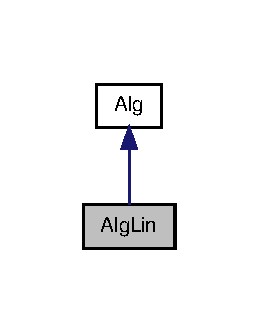
\includegraphics[width=124pt]{classAlgLin__inherit__graph}
\end{center}
\end{figure}


Collaboration diagram for AlgLin:
\nopagebreak
\begin{figure}[H]
\begin{center}
\leavevmode
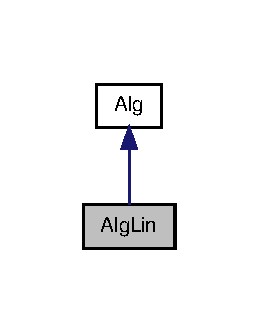
\includegraphics[width=124pt]{classAlgLin__coll__graph}
\end{center}
\end{figure}
\subsection*{Public Member Functions}
\begin{DoxyCompactItemize}
\item 
\hyperlink{classAlgLin_aff1317578ef31f6f1fd621015d6e6c5f}{AlgLin} (double in\_\-height, double in\_\-lenght, int in\_\-nx, int in\_\-ny, double in\_\-eps, char $\ast$in\_\-out\_\-name, int in\_\-count, double in\_\-t)
\begin{DoxyCompactList}\small\item\em Constructor. \end{DoxyCompactList}\item 
\hypertarget{classAlgLin_aed4bd552c5ef7d2b43e94c04286df633}{
void \hyperlink{classAlgLin_aed4bd552c5ef7d2b43e94c04286df633}{resolve\_\-r} ()}
\label{classAlgLin_aed4bd552c5ef7d2b43e94c04286df633}

\begin{DoxyCompactList}\small\item\em Function for recalculation of reciduals for all equations. \end{DoxyCompactList}\item 
void \hyperlink{classAlgLin_a7784f0707d7a081da5f85615f374df32}{resolve\_\-r} (int mode)
\item 
double \hyperlink{classAlgLin_a8323f1f45960e8d39184a61730fffffb}{find} (double $\ast$$\ast$a, double $\ast$$\ast$b, double $\ast$$\ast$c)
\begin{DoxyCompactList}\small\item\em Function to find method coefficient. \end{DoxyCompactList}\item 
double \hyperlink{classAlgLin_a0e6a96c3b072cb277bd7b1d4dd945472}{find} (int mode, double $\ast$$\ast$a, double $\ast$$\ast$b, double $\ast$$\ast$c)
\begin{DoxyCompactList}\small\item\em Function to find method coefficient for one equation. \end{DoxyCompactList}\item 
double $\ast$ \hyperlink{classAlgLin_ac5e5cd276c5be663d2d36ab92bf6ad83}{find\_\-all} (double $\ast$$\ast$a, double $\ast$$\ast$b, double $\ast$$\ast$c)
\item 
\hypertarget{classAlgLin_ad4c4596c11ad45040df273e022a508d7}{
void \hyperlink{classAlgLin_ad4c4596c11ad45040df273e022a508d7}{check\_\-result} ()}
\label{classAlgLin_ad4c4596c11ad45040df273e022a508d7}

\begin{DoxyCompactList}\small\item\em Function for independent verification of reciduals. \end{DoxyCompactList}\end{DoxyCompactItemize}


\subsection{Detailed Description}
Class for calculation linear equation of shallow water. 

This class contains specific for linear equations functionali 

\subsection{Constructor \& Destructor Documentation}
\hypertarget{classAlgLin_aff1317578ef31f6f1fd621015d6e6c5f}{
\index{AlgLin@{AlgLin}!AlgLin@{AlgLin}}
\index{AlgLin@{AlgLin}!AlgLin@{AlgLin}}
\subsubsection[{AlgLin}]{\setlength{\rightskip}{0pt plus 5cm}AlgLin::AlgLin (
\begin{DoxyParamCaption}
\item[{double}]{in\_\-height, }
\item[{double}]{in\_\-lenght, }
\item[{int}]{in\_\-nx, }
\item[{int}]{in\_\-ny, }
\item[{double}]{in\_\-eps, }
\item[{char $\ast$}]{in\_\-out\_\-name, }
\item[{int}]{in\_\-count, }
\item[{double}]{in\_\-t}
\end{DoxyParamCaption}
)\hspace{0.3cm}{\ttfamily  \mbox{[}inline\mbox{]}}}}
\label{classAlgLin_aff1317578ef31f6f1fd621015d6e6c5f}


Constructor. 


\begin{DoxyParams}{Parameters}
{\em in\_\-height} & Height calculation area \\
\hline
{\em in\_\-lenght} & Lenght calculation area \\
\hline
{\em in\_\-nx} & Count of Ox node \\
\hline
{\em in\_\-ny} & Count of Oy node \\
\hline
{\em in\_\-eps} & The accuracy of calculations \\
\hline
{\em in\_\-out\_\-name} & Output filename for save result \\
\hline
{\em count} & Count iteration by time \\
\hline
{\em in\_\-t} & Step by time \\
\hline
\end{DoxyParams}


\subsection{Member Function Documentation}
\hypertarget{classAlgLin_a0e6a96c3b072cb277bd7b1d4dd945472}{
\index{AlgLin@{AlgLin}!find@{find}}
\index{find@{find}!AlgLin@{AlgLin}}
\subsubsection[{find}]{\setlength{\rightskip}{0pt plus 5cm}double AlgLin::find (
\begin{DoxyParamCaption}
\item[{int}]{mode, }
\item[{double $\ast$$\ast$}]{a, }
\item[{double $\ast$$\ast$}]{b, }
\item[{double $\ast$$\ast$}]{c}
\end{DoxyParamCaption}
)\hspace{0.3cm}{\ttfamily  \mbox{[}virtual\mbox{]}}}}
\label{classAlgLin_a0e6a96c3b072cb277bd7b1d4dd945472}


Function to find method coefficient for one equation. 


\begin{DoxyParams}{Parameters}
{\em mode} & number of equation \\
\hline
{\em a} & array of data for first equation \\
\hline
{\em b} & array of data for second equation \\
\hline
{\em c} & array of data for third equation \\
\hline
\end{DoxyParams}


Implements \hyperlink{classAlg_a979d6df06027c6353b682662d8c514fc}{Alg}.

\hypertarget{classAlgLin_a8323f1f45960e8d39184a61730fffffb}{
\index{AlgLin@{AlgLin}!find@{find}}
\index{find@{find}!AlgLin@{AlgLin}}
\subsubsection[{find}]{\setlength{\rightskip}{0pt plus 5cm}double AlgLin::find (
\begin{DoxyParamCaption}
\item[{double $\ast$$\ast$}]{a, }
\item[{double $\ast$$\ast$}]{b, }
\item[{double $\ast$$\ast$}]{c}
\end{DoxyParamCaption}
)\hspace{0.3cm}{\ttfamily  \mbox{[}virtual\mbox{]}}}}
\label{classAlgLin_a8323f1f45960e8d39184a61730fffffb}


Function to find method coefficient. 


\begin{DoxyParams}{Parameters}
{\em a} & array of data for first equation \\
\hline
{\em b} & array of data for second equation \\
\hline
{\em c} & array of data for third equation \\
\hline
\end{DoxyParams}


Implements \hyperlink{classAlg_ada4ff3d2a0adb3b177d824e337158bfd}{Alg}.

\hypertarget{classAlgLin_ac5e5cd276c5be663d2d36ab92bf6ad83}{
\index{AlgLin@{AlgLin}!find\_\-all@{find\_\-all}}
\index{find\_\-all@{find\_\-all}!AlgLin@{AlgLin}}
\subsubsection[{find\_\-all}]{\setlength{\rightskip}{0pt plus 5cm}double $\ast$ AlgLin::find\_\-all (
\begin{DoxyParamCaption}
\item[{double $\ast$$\ast$}]{a, }
\item[{double $\ast$$\ast$}]{b, }
\item[{double $\ast$$\ast$}]{c}
\end{DoxyParamCaption}
)\hspace{0.3cm}{\ttfamily  \mbox{[}virtual\mbox{]}}}}
\label{classAlgLin_ac5e5cd276c5be663d2d36ab92bf6ad83}
not used 

Implements \hyperlink{classAlg_aef9cdfe539aed53c23222715c551e11e}{Alg}.

\hypertarget{classAlgLin_a7784f0707d7a081da5f85615f374df32}{
\index{AlgLin@{AlgLin}!resolve\_\-r@{resolve\_\-r}}
\index{resolve\_\-r@{resolve\_\-r}!AlgLin@{AlgLin}}
\subsubsection[{resolve\_\-r}]{\setlength{\rightskip}{0pt plus 5cm}void AlgLin::resolve\_\-r (
\begin{DoxyParamCaption}
\item[{int}]{mode}
\end{DoxyParamCaption}
)\hspace{0.3cm}{\ttfamily  \mbox{[}virtual\mbox{]}}}}
\label{classAlgLin_a7784f0707d7a081da5f85615f374df32}
Function for recalculation of reciduals for one equation 
\begin{DoxyParams}{Parameters}
{\em mode} & number of equation for recalculation \\
\hline
\end{DoxyParams}


Implements \hyperlink{classAlg_aa2436420b85976a48465408e9d86d425}{Alg}.



The documentation for this class was generated from the following files:\begin{DoxyCompactItemize}
\item 
/media/Documents/Documents/University/science/Numeric/Kurs/Kurs\_\-Linux/Kurs/src/alg\_\-lin.h\item 
/media/Documents/Documents/University/science/Numeric/Kurs/Kurs\_\-Linux/Kurs/src/alg\_\-lin.cpp\end{DoxyCompactItemize}

\hypertarget{classAlgNonlin}{
\section{AlgNonlin Class Reference}
\label{classAlgNonlin}\index{AlgNonlin@{AlgNonlin}}
}


Class for calculation nonlinear equation of shallow water.  




{\ttfamily \#include $<$alg\_\-nonlin.h$>$}



Inheritance diagram for AlgNonlin:
\nopagebreak
\begin{figure}[H]
\begin{center}
\leavevmode
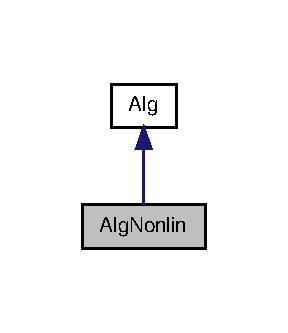
\includegraphics[width=138pt]{classAlgNonlin__inherit__graph}
\end{center}
\end{figure}


Collaboration diagram for AlgNonlin:
\nopagebreak
\begin{figure}[H]
\begin{center}
\leavevmode
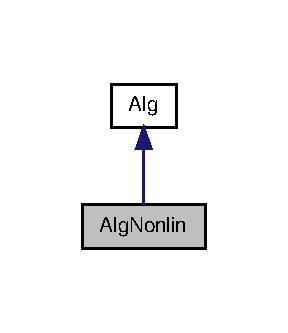
\includegraphics[width=138pt]{classAlgNonlin__coll__graph}
\end{center}
\end{figure}
\subsection*{Public Member Functions}
\begin{DoxyCompactItemize}
\item 
\hyperlink{classAlgNonlin_a3a4b7b0afb7e2ef2cc3f09b6d35fec42}{AlgNonlin} (double in\_\-height, double in\_\-lenght, int in\_\-nx, int in\_\-ny, double in\_\-eps, char $\ast$in\_\-out\_\-name, int in\_\-count, double in\_\-t)
\begin{DoxyCompactList}\small\item\em Constructor. \end{DoxyCompactList}\item 
\hypertarget{classAlgNonlin_a575576e90c96d93b28debdf30f51e741}{
void \hyperlink{classAlgNonlin_a575576e90c96d93b28debdf30f51e741}{resolve\_\-r} ()}
\label{classAlgNonlin_a575576e90c96d93b28debdf30f51e741}

\begin{DoxyCompactList}\small\item\em Function for recalculation of reciduals for all equations. \end{DoxyCompactList}\item 
void \hyperlink{classAlgNonlin_a28bbb13e708a32cf4f191db56325e52c}{resolve\_\-r} (int mode)
\item 
double \hyperlink{classAlgNonlin_ae7c521438daed488cd69b131292f2a8a}{find} (double $\ast$$\ast$a, double $\ast$$\ast$b, double $\ast$$\ast$c)
\begin{DoxyCompactList}\small\item\em Function to find method coefficient. \end{DoxyCompactList}\item 
double \hyperlink{classAlgNonlin_a164094279ad86962c650221b112c9223}{find} (int mode, double $\ast$$\ast$a, double $\ast$$\ast$b, double $\ast$$\ast$c)
\begin{DoxyCompactList}\small\item\em Function to find method coefficient for one equation. \end{DoxyCompactList}\item 
double $\ast$ \hyperlink{classAlgNonlin_a3f3bdece3eb2ccaffeb7c19bd318121e}{find\_\-all} (double $\ast$$\ast$a, double $\ast$$\ast$b, double $\ast$$\ast$c)
\item 
\hypertarget{classAlgNonlin_a885ddfe1f2181d777f98503d66480e1c}{
void \hyperlink{classAlgNonlin_a885ddfe1f2181d777f98503d66480e1c}{check\_\-result} ()}
\label{classAlgNonlin_a885ddfe1f2181d777f98503d66480e1c}

\begin{DoxyCompactList}\small\item\em Function for independent verification of reciduals. \end{DoxyCompactList}\end{DoxyCompactItemize}


\subsection{Detailed Description}
Class for calculation nonlinear equation of shallow water. 

This class contains specific for nonlinear equations functionali 

\subsection{Constructor \& Destructor Documentation}
\hypertarget{classAlgNonlin_a3a4b7b0afb7e2ef2cc3f09b6d35fec42}{
\index{AlgNonlin@{AlgNonlin}!AlgNonlin@{AlgNonlin}}
\index{AlgNonlin@{AlgNonlin}!AlgNonlin@{AlgNonlin}}
\subsubsection[{AlgNonlin}]{\setlength{\rightskip}{0pt plus 5cm}AlgNonlin::AlgNonlin (
\begin{DoxyParamCaption}
\item[{double}]{in\_\-height, }
\item[{double}]{in\_\-lenght, }
\item[{int}]{in\_\-nx, }
\item[{int}]{in\_\-ny, }
\item[{double}]{in\_\-eps, }
\item[{char $\ast$}]{in\_\-out\_\-name, }
\item[{int}]{in\_\-count, }
\item[{double}]{in\_\-t}
\end{DoxyParamCaption}
)\hspace{0.3cm}{\ttfamily  \mbox{[}inline\mbox{]}}}}
\label{classAlgNonlin_a3a4b7b0afb7e2ef2cc3f09b6d35fec42}


Constructor. 


\begin{DoxyParams}{Parameters}
{\em in\_\-height} & Height calculation area \\
\hline
{\em in\_\-lenght} & Lenght calculation area \\
\hline
{\em in\_\-nx} & Count of Ox node \\
\hline
{\em in\_\-ny} & Count of Oy node \\
\hline
{\em in\_\-eps} & The accuracy of calculations \\
\hline
{\em in\_\-out\_\-name} & Output filename for save result \\
\hline
{\em count} & Count iteration by time \\
\hline
{\em in\_\-t} & Step by time \\
\hline
\end{DoxyParams}


\subsection{Member Function Documentation}
\hypertarget{classAlgNonlin_a164094279ad86962c650221b112c9223}{
\index{AlgNonlin@{AlgNonlin}!find@{find}}
\index{find@{find}!AlgNonlin@{AlgNonlin}}
\subsubsection[{find}]{\setlength{\rightskip}{0pt plus 5cm}double AlgNonlin::find (
\begin{DoxyParamCaption}
\item[{int}]{mode, }
\item[{double $\ast$$\ast$}]{a, }
\item[{double $\ast$$\ast$}]{b, }
\item[{double $\ast$$\ast$}]{c}
\end{DoxyParamCaption}
)\hspace{0.3cm}{\ttfamily  \mbox{[}virtual\mbox{]}}}}
\label{classAlgNonlin_a164094279ad86962c650221b112c9223}


Function to find method coefficient for one equation. 


\begin{DoxyParams}{Parameters}
{\em mode} & number of equation \\
\hline
{\em a} & array of data for first equation \\
\hline
{\em b} & array of data for second equation \\
\hline
{\em c} & array of data for third equation \\
\hline
\end{DoxyParams}


Implements \hyperlink{classAlg_a979d6df06027c6353b682662d8c514fc}{Alg}.

\hypertarget{classAlgNonlin_ae7c521438daed488cd69b131292f2a8a}{
\index{AlgNonlin@{AlgNonlin}!find@{find}}
\index{find@{find}!AlgNonlin@{AlgNonlin}}
\subsubsection[{find}]{\setlength{\rightskip}{0pt plus 5cm}double AlgNonlin::find (
\begin{DoxyParamCaption}
\item[{double $\ast$$\ast$}]{a, }
\item[{double $\ast$$\ast$}]{b, }
\item[{double $\ast$$\ast$}]{c}
\end{DoxyParamCaption}
)\hspace{0.3cm}{\ttfamily  \mbox{[}virtual\mbox{]}}}}
\label{classAlgNonlin_ae7c521438daed488cd69b131292f2a8a}


Function to find method coefficient. 


\begin{DoxyParams}{Parameters}
{\em a} & array of data for first equation \\
\hline
{\em b} & array of data for second equation \\
\hline
{\em c} & array of data for third equation \\
\hline
\end{DoxyParams}


Implements \hyperlink{classAlg_ada4ff3d2a0adb3b177d824e337158bfd}{Alg}.

\hypertarget{classAlgNonlin_a3f3bdece3eb2ccaffeb7c19bd318121e}{
\index{AlgNonlin@{AlgNonlin}!find\_\-all@{find\_\-all}}
\index{find\_\-all@{find\_\-all}!AlgNonlin@{AlgNonlin}}
\subsubsection[{find\_\-all}]{\setlength{\rightskip}{0pt plus 5cm}double $\ast$ AlgNonlin::find\_\-all (
\begin{DoxyParamCaption}
\item[{double $\ast$$\ast$}]{a, }
\item[{double $\ast$$\ast$}]{b, }
\item[{double $\ast$$\ast$}]{c}
\end{DoxyParamCaption}
)\hspace{0.3cm}{\ttfamily  \mbox{[}virtual\mbox{]}}}}
\label{classAlgNonlin_a3f3bdece3eb2ccaffeb7c19bd318121e}
not used 

Implements \hyperlink{classAlg_aef9cdfe539aed53c23222715c551e11e}{Alg}.

\hypertarget{classAlgNonlin_a28bbb13e708a32cf4f191db56325e52c}{
\index{AlgNonlin@{AlgNonlin}!resolve\_\-r@{resolve\_\-r}}
\index{resolve\_\-r@{resolve\_\-r}!AlgNonlin@{AlgNonlin}}
\subsubsection[{resolve\_\-r}]{\setlength{\rightskip}{0pt plus 5cm}void AlgNonlin::resolve\_\-r (
\begin{DoxyParamCaption}
\item[{int}]{mode}
\end{DoxyParamCaption}
)\hspace{0.3cm}{\ttfamily  \mbox{[}virtual\mbox{]}}}}
\label{classAlgNonlin_a28bbb13e708a32cf4f191db56325e52c}
Function for recalculation of reciduals for one equation 
\begin{DoxyParams}{Parameters}
{\em mode} & number of equation for recalculation \\
\hline
\end{DoxyParams}


Implements \hyperlink{classAlg_aa2436420b85976a48465408e9d86d425}{Alg}.



The documentation for this class was generated from the following files:\begin{DoxyCompactItemize}
\item 
/media/Documents/Documents/University/science/Numeric/Kurs/Kurs\_\-Linux/Kurs/src/alg\_\-nonlin.h\item 
/media/Documents/Documents/University/science/Numeric/Kurs/Kurs\_\-Linux/Kurs/src/alg\_\-nonlin.cpp\end{DoxyCompactItemize}

\hypertarget{classComparer}{
\section{Comparer Class Reference}
\label{classComparer}\index{Comparer@{Comparer}}
}


Class to comparison of data files.  




{\ttfamily \#include $<$comparer.h$>$}

\subsection*{Public Member Functions}
\begin{DoxyCompactItemize}
\item 
\hyperlink{classComparer_a7dacd3d3d4334c35520ed23dee0b80b8}{Comparer} (int nx, int ny, double hx, double hy, int time)
\begin{DoxyCompactList}\small\item\em Constructor. \end{DoxyCompactList}\item 
void \hyperlink{classComparer_a7e557fdd48f24aa1f916660f314c4428}{delta} (char $\ast$file1, char $\ast$file2, char $\ast$result)
\begin{DoxyCompactList}\small\item\em Function to comparison. \end{DoxyCompactList}\end{DoxyCompactItemize}


\subsection{Detailed Description}
Class to comparison of data files. 

\subsection{Constructor \& Destructor Documentation}
\hypertarget{classComparer_a7dacd3d3d4334c35520ed23dee0b80b8}{
\index{Comparer@{Comparer}!Comparer@{Comparer}}
\index{Comparer@{Comparer}!Comparer@{Comparer}}
\subsubsection[{Comparer}]{\setlength{\rightskip}{0pt plus 5cm}Comparer::Comparer (
\begin{DoxyParamCaption}
\item[{int}]{nx, }
\item[{int}]{ny, }
\item[{double}]{hx, }
\item[{double}]{hy, }
\item[{int}]{time}
\end{DoxyParamCaption}
)}}
\label{classComparer_a7dacd3d3d4334c35520ed23dee0b80b8}


Constructor. 


\begin{DoxyParams}{Parameters}
{\em nx} & num node by Ox \\
\hline
{\em ny} & num node by Oy \\
\hline
{\em hx} & step by Ox \\
\hline
{\em hy} & step by Oy \\
\hline
{\em time} & count steps by time \\
\hline
\end{DoxyParams}


\subsection{Member Function Documentation}
\hypertarget{classComparer_a7e557fdd48f24aa1f916660f314c4428}{
\index{Comparer@{Comparer}!delta@{delta}}
\index{delta@{delta}!Comparer@{Comparer}}
\subsubsection[{delta}]{\setlength{\rightskip}{0pt plus 5cm}void Comparer::delta (
\begin{DoxyParamCaption}
\item[{char $\ast$}]{file1, }
\item[{char $\ast$}]{file2, }
\item[{char $\ast$}]{result}
\end{DoxyParamCaption}
)}}
\label{classComparer_a7e557fdd48f24aa1f916660f314c4428}


Function to comparison. 


\begin{DoxyParams}{Parameters}
{\em file1} & first file \\
\hline
{\em file2} & second file \\
\hline
{\em result} & file name to output \\
\hline
\end{DoxyParams}


The documentation for this class was generated from the following files:\begin{DoxyCompactItemize}
\item 
/media/Documents/Documents/University/science/Numeric/Kurs/Kurs\_\-Linux/Kurs/src/comparer.h\item 
/media/Documents/Documents/University/science/Numeric/Kurs/Kurs\_\-Linux/Kurs/src/comparer.cpp\end{DoxyCompactItemize}

\chapter{File Documentation}
\hypertarget{definition_8h}{
\section{/media/Documents/Documents/University/science/Numeric/Kurs/Kurs\_\-Linux/Kurs/src/definition.h File Reference}
\label{definition_8h}\index{/media/Documents/Documents/University/science/Numeric/Kurs/Kurs\_\-Linux/Kurs/src/definition.h@{/media/Documents/Documents/University/science/Numeric/Kurs/Kurs\_\-Linux/Kurs/src/definition.h}}
}
This graph shows which files directly or indirectly include this file:
\nopagebreak
\begin{figure}[H]
\begin{center}
\leavevmode
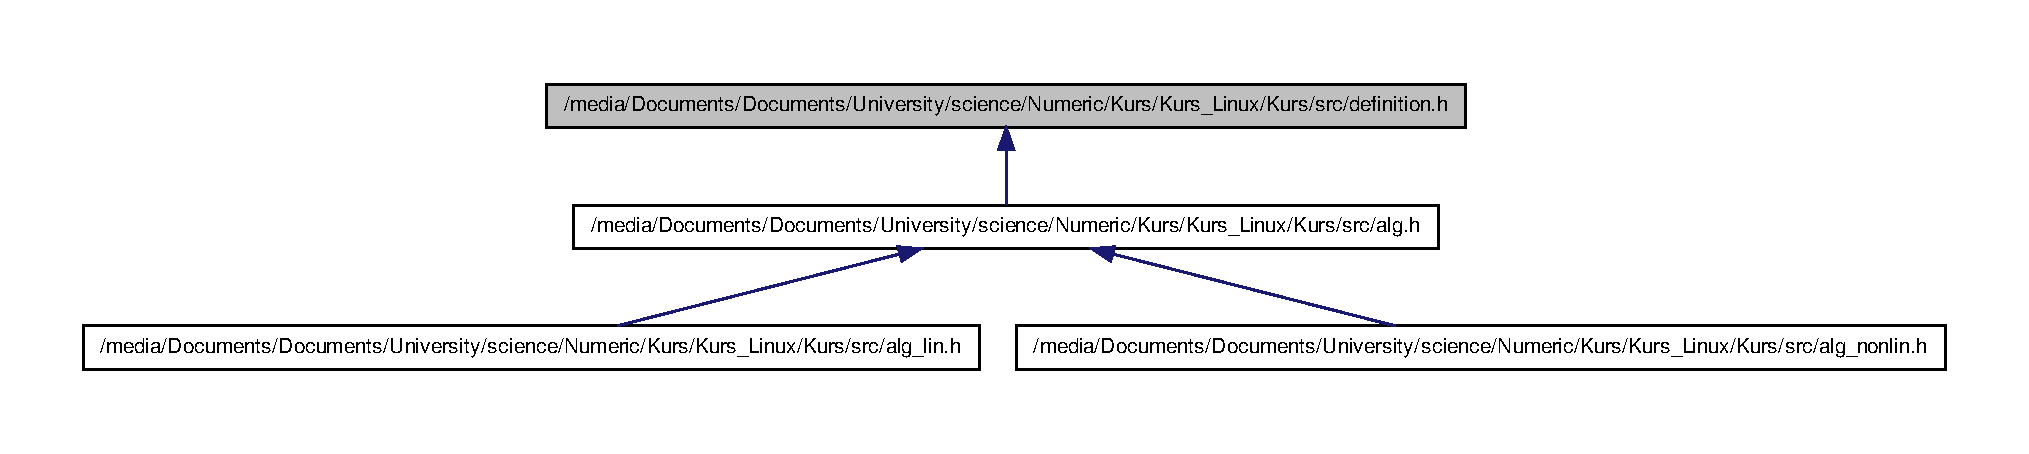
\includegraphics[width=400pt]{definition_8h__dep__incl}
\end{center}
\end{figure}
\subsection*{Defines}
\begin{DoxyCompactItemize}
\item 
\#define \hyperlink{definition_8h_a60a5ae0f649d015e57358b74379701c5}{centering\_\-wave}(height, grad, i, j)~height$\ast$exp(-\/grad$\ast$(((double)i/nx-\/0.5)$\ast$((double)i/nx-\/0.5)))
\begin{DoxyCompactList}\small\item\em Long Ox centering wave. \end{DoxyCompactList}\item 
\#define \hyperlink{definition_8h_a8394da0c2596dfaf6df870fe488596da}{wave}(height, grad, i, j, shift)~height$\ast$exp(-\/grad$\ast$(((double)i/nx-\/shift)$\ast$((double)i/nx-\/shift)))
\begin{DoxyCompactList}\small\item\em Long Ox wave. \end{DoxyCompactList}\item 
\#define \hyperlink{definition_8h_a5e750d7a713925405ab12b788fcde3b0}{centering\_\-drop}(height, grad, i, j)~height$\ast$exp(-\/grad$\ast$(((double)i/nx-\/0.5)$\ast$((double)i/nx-\/0.5)+((double)j/ny-\/0.5)$\ast$((double)j/ny-\/0.5)))
\begin{DoxyCompactList}\small\item\em Small centering drop. \end{DoxyCompactList}\item 
\#define \hyperlink{definition_8h_aeb863677d329117f4b386ddfade29024}{drop}(height, grad, i, j, shiftX, shiftY)~height$\ast$exp(-\/grad$\ast$(((double)i/nx-\/shiftX)$\ast$((double)i/nx-\/shiftX)+((double)j/ny-\/shiftY)$\ast$((double)j/ny-\/shiftY)))
\begin{DoxyCompactList}\small\item\em Small drop. \end{DoxyCompactList}\item 
\#define \hyperlink{definition_8h_a54316f8a22a09747db6f077fadae87cf}{stair}(i, j)~if(i$<$nx/10)\{return 0;\}
\begin{DoxyCompactList}\small\item\em Bottom function. \end{DoxyCompactList}\item 
\#define \hyperlink{definition_8h_ab0d868f50ee592f363693151df01be37}{stair\_\-shift}(i, j, shift)~if(i$<$nx/shift)\{return 0;\}
\begin{DoxyCompactList}\small\item\em Bottom function. \end{DoxyCompactList}\item 
\#define \hyperlink{definition_8h_ab09fd0612528376375b99647764df0cf}{rise}(i, j)~if(i$<$nx/3\&\&i$>$nx/5)\{return 0.01-\/(nx/3-\/i)$\ast$0.001;\}; if(i$<$=nx/5)\{return 0.01-\/(nx/3-\/nx/5)$\ast$0.001;\}
\begin{DoxyCompactList}\small\item\em Bottom function. \end{DoxyCompactList}\item 
\#define \hyperlink{definition_8h_a29a35654ab5aa98a523c1147e69cb9d1}{cylinder}(i, j)~if(sqrt((i$\ast$hx-\/0.5)$\ast$(i$\ast$hx-\/0.5)+(j$\ast$hy-\/0.5)$\ast$(j$\ast$hy-\/0.5))$<$0.05)\{return 0.2;\}
\begin{DoxyCompactList}\small\item\em Bottom function. \end{DoxyCompactList}\item 
\hypertarget{definition_8h_a3d8c9c145887af5174ba4cc6789862ad}{
\#define \hyperlink{definition_8h_a3d8c9c145887af5174ba4cc6789862ad}{TAU}~0}
\label{definition_8h_a3d8c9c145887af5174ba4cc6789862ad}

\begin{DoxyCompactList}\small\item\em Constants for TAU mode in solve process. \end{DoxyCompactList}\item 
\hypertarget{definition_8h_ad22c94c78a741ad767300c9b586ac4f8}{
\#define \hyperlink{definition_8h_ad22c94c78a741ad767300c9b586ac4f8}{ALFA}~1}
\label{definition_8h_ad22c94c78a741ad767300c9b586ac4f8}

\begin{DoxyCompactList}\small\item\em Constants for ALFA mode in solve process. \end{DoxyCompactList}\item 
\hypertarget{definition_8h_a167d2c0ec9b943d55f2124f7442b2f6d}{
\#define \hyperlink{definition_8h_a167d2c0ec9b943d55f2124f7442b2f6d}{g}~9.8}
\label{definition_8h_a167d2c0ec9b943d55f2124f7442b2f6d}

\begin{DoxyCompactList}\small\item\em Constants for g. \end{DoxyCompactList}\end{DoxyCompactItemize}


\subsection{Detailed Description}
This file contains the definitions of macro, which describe forms of free surface of fluid, form of bottom and some constants. 

\subsection{Define Documentation}
\hypertarget{definition_8h_a5e750d7a713925405ab12b788fcde3b0}{
\index{definition.h@{definition.h}!centering\_\-drop@{centering\_\-drop}}
\index{centering\_\-drop@{centering\_\-drop}!definition.h@{definition.h}}
\subsubsection[{centering\_\-drop}]{\setlength{\rightskip}{0pt plus 5cm}\#define centering\_\-drop(
\begin{DoxyParamCaption}
\item[{}]{height, }
\item[{}]{grad, }
\item[{}]{i, }
\item[{}]{j}
\end{DoxyParamCaption}
)~height$\ast$exp(-\/grad$\ast$(((double)i/nx-\/0.5)$\ast$((double)i/nx-\/0.5)+((double)j/ny-\/0.5)$\ast$((double)j/ny-\/0.5)))}}
\label{definition_8h_a5e750d7a713925405ab12b788fcde3b0}


Small centering drop. 


\begin{DoxyParams}{Parameters}
{\em height} & height of drop \\
\hline
{\em grad} & degree of steepness of the ascent \\
\hline
\end{DoxyParams}
\hypertarget{definition_8h_a60a5ae0f649d015e57358b74379701c5}{
\index{definition.h@{definition.h}!centering\_\-wave@{centering\_\-wave}}
\index{centering\_\-wave@{centering\_\-wave}!definition.h@{definition.h}}
\subsubsection[{centering\_\-wave}]{\setlength{\rightskip}{0pt plus 5cm}\#define centering\_\-wave(
\begin{DoxyParamCaption}
\item[{}]{height, }
\item[{}]{grad, }
\item[{}]{i, }
\item[{}]{j}
\end{DoxyParamCaption}
)~height$\ast$exp(-\/grad$\ast$(((double)i/nx-\/0.5)$\ast$((double)i/nx-\/0.5)))}}
\label{definition_8h_a60a5ae0f649d015e57358b74379701c5}


Long Ox centering wave. 


\begin{DoxyParams}{Parameters}
{\em height} & height of wave \\
\hline
{\em grad} & degree of steepness of the ascent \\
\hline
\end{DoxyParams}
\hypertarget{definition_8h_a29a35654ab5aa98a523c1147e69cb9d1}{
\index{definition.h@{definition.h}!cylinder@{cylinder}}
\index{cylinder@{cylinder}!definition.h@{definition.h}}
\subsubsection[{cylinder}]{\setlength{\rightskip}{0pt plus 5cm}\#define cylinder(
\begin{DoxyParamCaption}
\item[{}]{i, }
\item[{}]{j}
\end{DoxyParamCaption}
)~if(sqrt((i$\ast$hx-\/0.5)$\ast$(i$\ast$hx-\/0.5)+(j$\ast$hy-\/0.5)$\ast$(j$\ast$hy-\/0.5))$<$0.05)\{return 0.2;\}}}
\label{definition_8h_a29a35654ab5aa98a523c1147e69cb9d1}


Bottom function. 


\begin{DoxyCode}
 cylinder
       --
       ||
 ------  -------
\end{DoxyCode}
 \hypertarget{definition_8h_aeb863677d329117f4b386ddfade29024}{
\index{definition.h@{definition.h}!drop@{drop}}
\index{drop@{drop}!definition.h@{definition.h}}
\subsubsection[{drop}]{\setlength{\rightskip}{0pt plus 5cm}\#define drop(
\begin{DoxyParamCaption}
\item[{}]{height, }
\item[{}]{grad, }
\item[{}]{i, }
\item[{}]{j, }
\item[{}]{shiftX, }
\item[{}]{shiftY}
\end{DoxyParamCaption}
)~height$\ast$exp(-\/grad$\ast$(((double)i/nx-\/shiftX)$\ast$((double)i/nx-\/shiftX)+((double)j/ny-\/shiftY)$\ast$((double)j/ny-\/shiftY)))}}
\label{definition_8h_aeb863677d329117f4b386ddfade29024}


Small drop. 


\begin{DoxyParams}{Parameters}
{\em height} & height of drop \\
\hline
{\em grad} & degree of steepness of the ascent \\
\hline
{\em shiftX} & offset from the origin of Ox \\
\hline
{\em shiftY} & offset from the origin of Oy \\
\hline
\end{DoxyParams}
\hypertarget{definition_8h_ab09fd0612528376375b99647764df0cf}{
\index{definition.h@{definition.h}!rise@{rise}}
\index{rise@{rise}!definition.h@{definition.h}}
\subsubsection[{rise}]{\setlength{\rightskip}{0pt plus 5cm}\#define rise(
\begin{DoxyParamCaption}
\item[{}]{i, }
\item[{}]{j}
\end{DoxyParamCaption}
)~if(i$<$nx/3\&\&i$>$nx/5)\{return 0.01-\/(nx/3-\/i)$\ast$0.001;\}; if(i$<$=nx/5)\{return 0.01-\/(nx/3-\/nx/5)$\ast$0.001;\}}}
\label{definition_8h_ab09fd0612528376375b99647764df0cf}


Bottom function. 


\begin{DoxyCode}
 rise
 ----
     -
      -
       --------
\end{DoxyCode}
 \hypertarget{definition_8h_a54316f8a22a09747db6f077fadae87cf}{
\index{definition.h@{definition.h}!stair@{stair}}
\index{stair@{stair}!definition.h@{definition.h}}
\subsubsection[{stair}]{\setlength{\rightskip}{0pt plus 5cm}\#define stair(
\begin{DoxyParamCaption}
\item[{}]{i, }
\item[{}]{j}
\end{DoxyParamCaption}
)~if(i$<$nx/10)\{return 0;\}}}
\label{definition_8h_a54316f8a22a09747db6f077fadae87cf}


Bottom function. 


\begin{DoxyCode}
 stair
 -----
     |
     |---------
\end{DoxyCode}
 \hypertarget{definition_8h_ab0d868f50ee592f363693151df01be37}{
\index{definition.h@{definition.h}!stair\_\-shift@{stair\_\-shift}}
\index{stair\_\-shift@{stair\_\-shift}!definition.h@{definition.h}}
\subsubsection[{stair\_\-shift}]{\setlength{\rightskip}{0pt plus 5cm}\#define stair\_\-shift(
\begin{DoxyParamCaption}
\item[{}]{i, }
\item[{}]{j, }
\item[{}]{shift}
\end{DoxyParamCaption}
)~if(i$<$nx/shift)\{return 0;\}}}
\label{definition_8h_ab0d868f50ee592f363693151df01be37}


Bottom function. 


\begin{DoxyCode}
 stair
 -----
     |
     |---------
\end{DoxyCode}
 \hypertarget{definition_8h_a8394da0c2596dfaf6df870fe488596da}{
\index{definition.h@{definition.h}!wave@{wave}}
\index{wave@{wave}!definition.h@{definition.h}}
\subsubsection[{wave}]{\setlength{\rightskip}{0pt plus 5cm}\#define wave(
\begin{DoxyParamCaption}
\item[{}]{height, }
\item[{}]{grad, }
\item[{}]{i, }
\item[{}]{j, }
\item[{}]{shift}
\end{DoxyParamCaption}
)~height$\ast$exp(-\/grad$\ast$(((double)i/nx-\/shift)$\ast$((double)i/nx-\/shift)))}}
\label{definition_8h_a8394da0c2596dfaf6df870fe488596da}


Long Ox wave. 


\begin{DoxyParams}{Parameters}
{\em height} & height of wave \\
\hline
{\em grad} & degree of steepness of the ascent \\
\hline
{\em shift} & offset from the origin of coordinates \\
\hline
\end{DoxyParams}

\printindex
\end{document}
